
%% jan. 4, 2011  items to fix:
%% notation for math and reference to images.
%% how include eps figures.
%% make all the little figures (search for eps) in a common, nice matlab way for the
%% example filtering operations.

%\setcounter{chapter}{5}
\chapter{Color}
\label{chapter:color}

%\reviewcomment{Figures need reformating.}

\section{Introduction}

There are many benefits to sensing color.  Color differences let us
check whether fruit is ripe, tell whether a child is sick by looking
at small changes in the color of the skin, and find objects in
clutter.  

We'll begin our study of color by describing the physical properties of light that lead to the perception of different colors.  Then we'll describe how humans and machines sense colors, and how to build a system to match the colors perceived by an observer.  We'll briefly describe how to represent color--different color coordinate systems.  Finally, we'll describe how spatial resolution and color interact.


\section{Color Physics}


Isaac Newton revealed several intrinsic
properties of light in experiments summarized by his drawing in
\fig{\ref{fig:prism}}. A pinhole of sunlight enters through the
window shade, and a lens focuses the light onto a prism.  The prism
then divides the white light into many different colors.  These
colors are elemental: if one of
the component colors is passed through a second prism, it doesn't
split into further components.


\begin{figure}[htpb!]
\centerline{
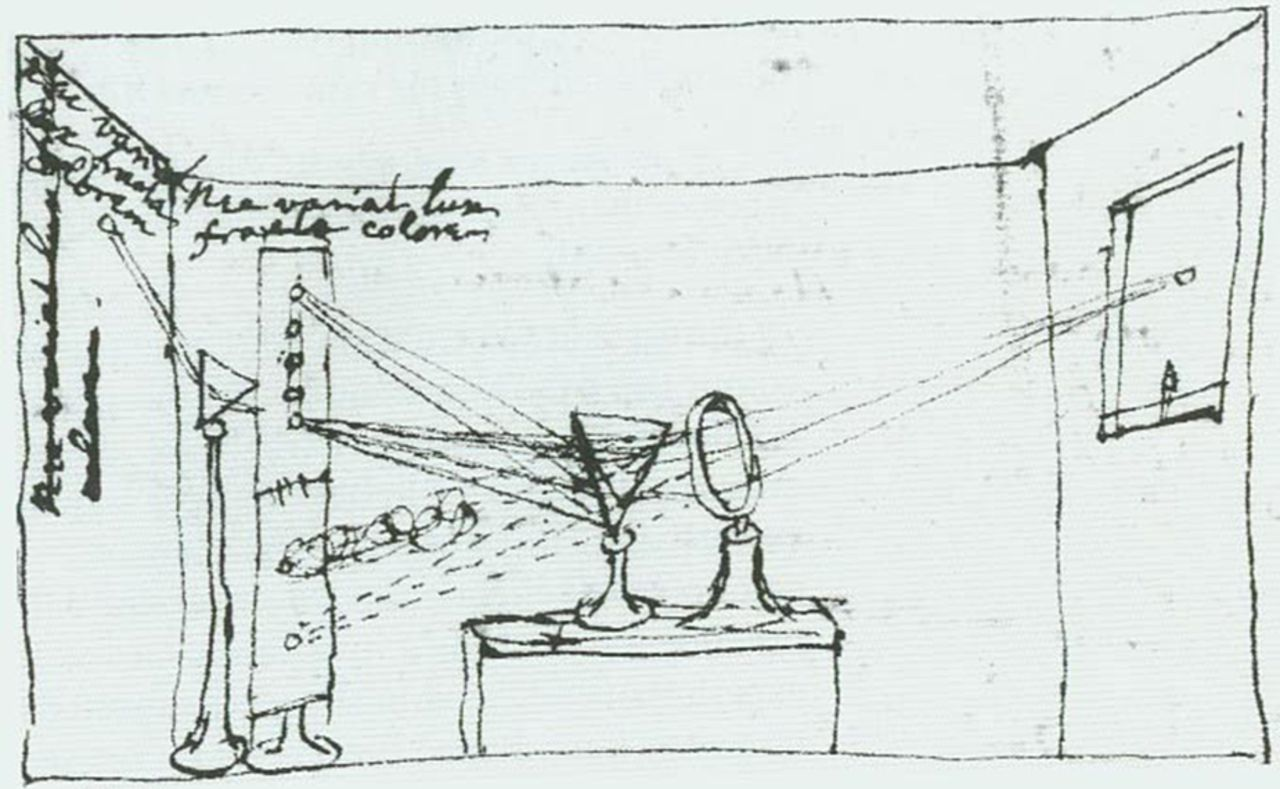
\includegraphics[width=.9\linewidth]{figures/color/newtonDrawing.jpg}
}
\caption{Isaac Newton's illustration of experiments with light \cite{Fara2015}.  White
light enters from a hole in the window shade at the right, where it is
focused with a lens and then passes through the first
prism.  The prism separates the white light into different colors by
bending each color a different amount.  The second prism in the
drawing demonstrates that those colors are elemental:  as an individual
color passes through the second prism, the light doesn't break into
other colors.}
\label{fig:prism}
\end{figure}


Our understanding of light and color explains such experiments.  Light
is a mixture of electromagnetic waves of different wavelengths.
Sunlight has a broad distribution of
light of the visible wavelengths.  At an air/glass interface, light
bends in a wavelength-dependent manner, so a prism disperses the
different wavelength components of sunlight into different angles, and
we see different wavelengths of light as different colors.  
Our eyes are sensitive to only the narrow band of that electromagnetic
spectrum, the visible light, from approximately 400 nm 
to 700 nm, which appears blue to deep red, respectively.




The bending of light at a material boundary is called {\bf refraction}, and
its wavelength dependence lets the prism separate white light into its
component colors.  A second way to separate light into its spectral
components is through {\bf diffraction}, where constructive
interference of scattered light occurs in different directions for
different wavelengths of light. 
\marginnote{Newton understood that white light could be decomposed into different colors and invented the term {\bf spectrum}.}

\Fig{\ref{fig:colorWavelengths}}{a} 
shows a simple spectrograph, an apparatus to reveal the spectrum of light, based on
diffraction from a compact disk (CD) \cite{spectrometer}.  Light passes through the slit at
the right, and strikes a CD (with a track pitch of about 1,600 nm).
Constructive interference from the light waves striking the CD tracks
will occur at a different angle for each wavelength of the light, yielding
a separation of the different wavelengths of light according to their
angle of diffraction.  The diffracted 
light can be viewed,   \fig{\ref{fig:colorWavelengths}}{b}, 
or photographed through the hole at the bottom
left of the photograph.  The spectrograph gives an immediate visual
representation of the spectral components of colors in the world. Some examples are shown in \fig{\ref{fig:examples1}}.



\begin{figure}[t]
\centerline{
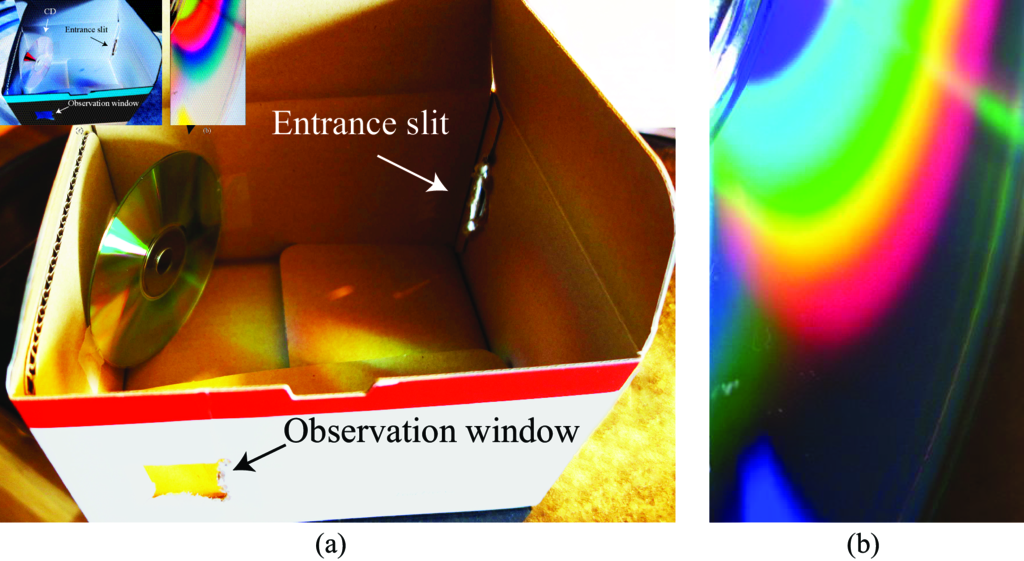
\includegraphics[width=1.0\linewidth]{figures/color/cd_spectrometer_setup.eps}
}
%\centerline{
%\sublabel{a}{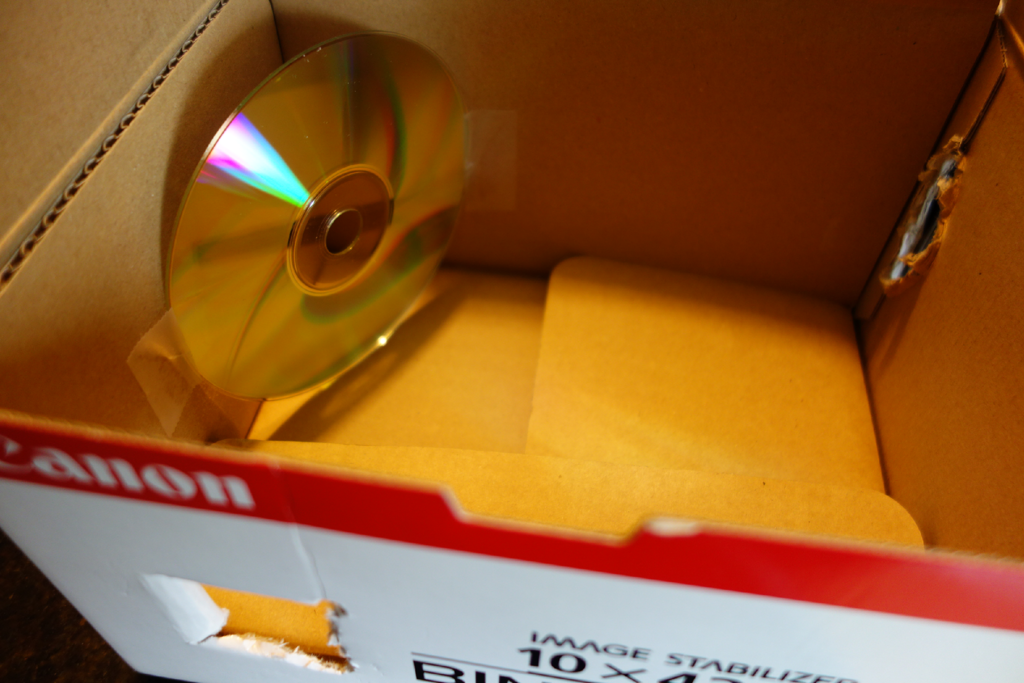
\epsfig{file=figures/color/cdSpectrograph.eps,width=3in}}
%\sublabel{a}{\epsfig{file=figures/color/spectrometer2.jpg,width=3in}}
%\sublabel{b}{
\epsfig{file=figures/color/rainbow.eps,width=1.5in}}}
\caption{(a) A simple spectrograph.
  Slit at right accepts light from primarily one object in the world.
  Light diffracted by the CD is viewed from the hole at the bottom
  left.  (b) The bending by diffraction is wavelength dependent, and the
  light from a given direction is broken into its spectral components. We indicate the location of the CD in the picture just in case our youngest readers have not seen one.}
\label{fig:colorWavelengths}
\end{figure}




\begin{figure}
\centerline{
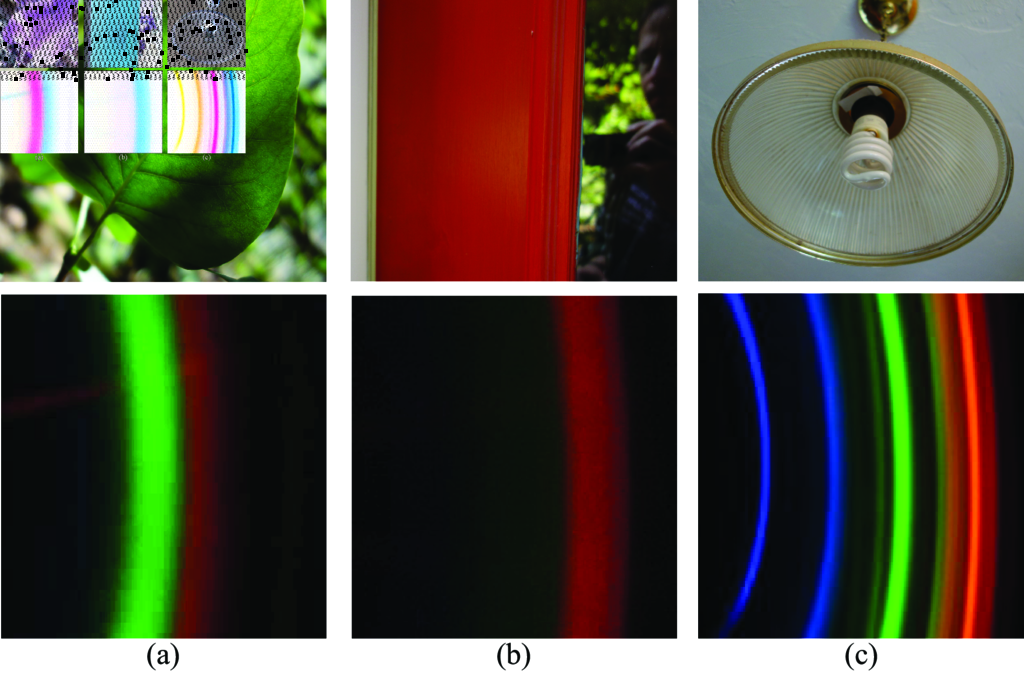
\includegraphics[width=1.0\linewidth]{figures/color/lightspectra_objects.eps}
}
%\sublabel{a}{\centerline{
%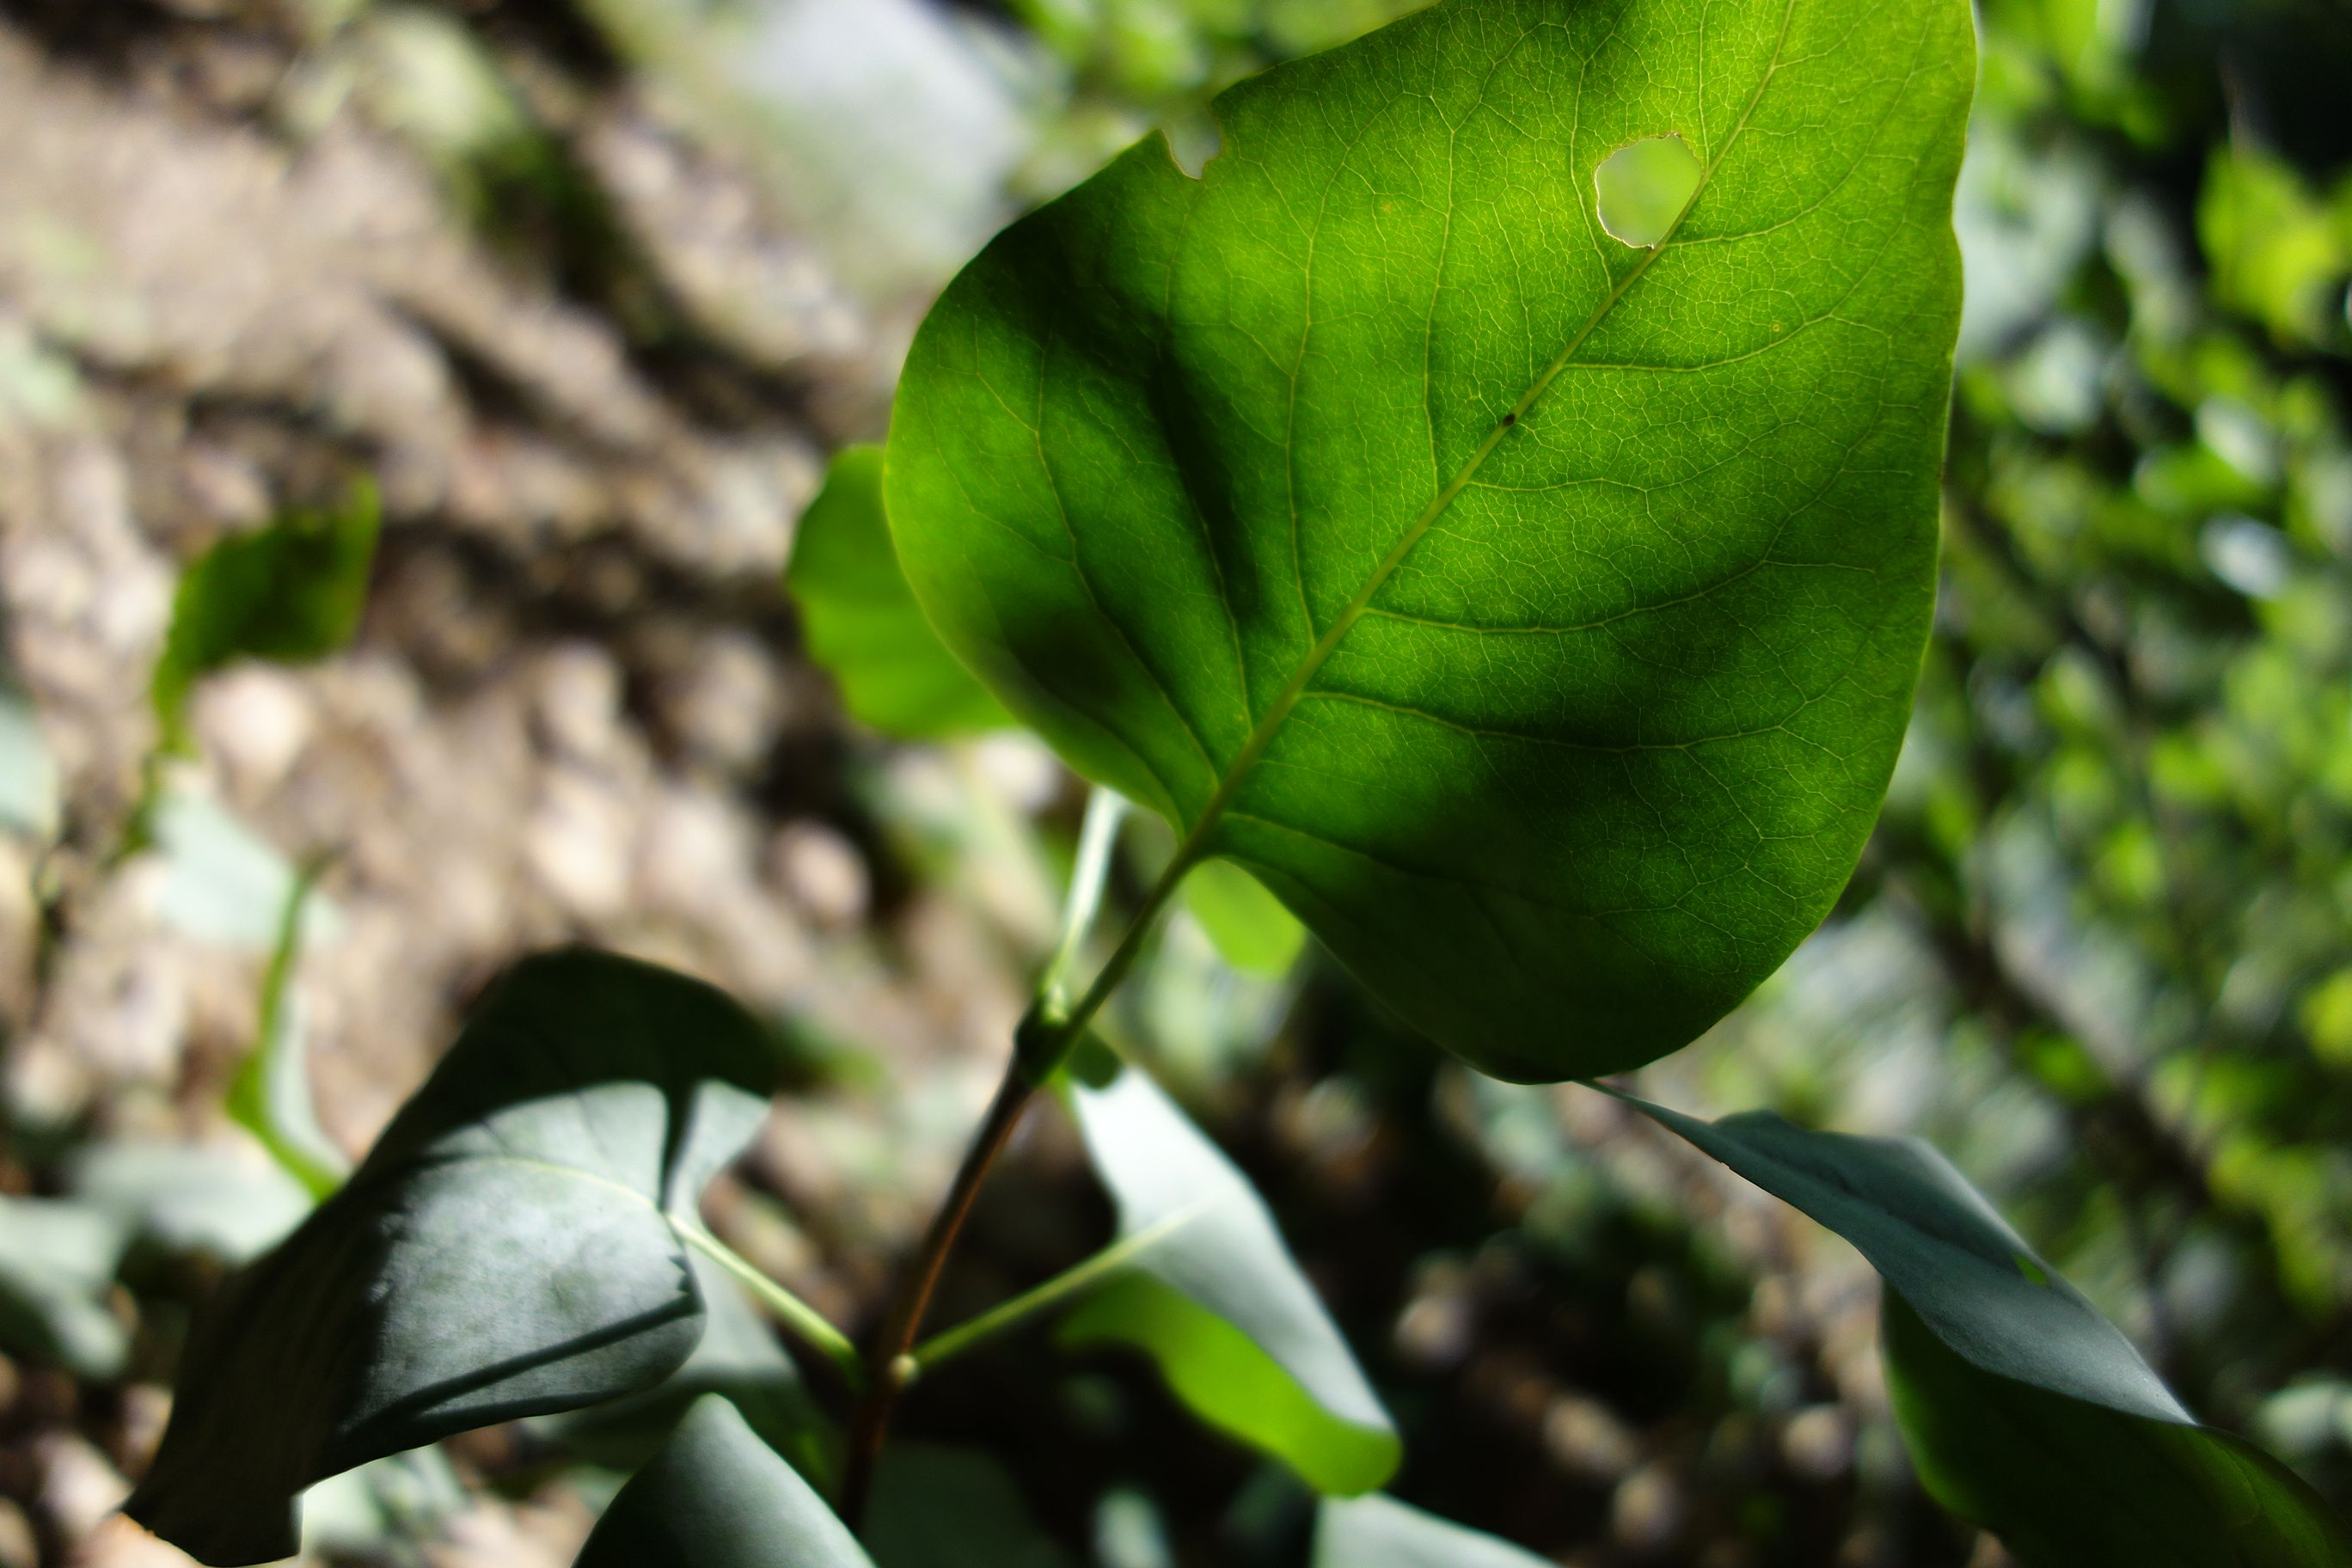
\epsfig{file=figures/color/DSC00780.jpg,width=1.7in}
%
\epsfig{file=figures/color/leafspec.eps,width=1.05in}
%}}
%\sublabel{b}{\centerline{
%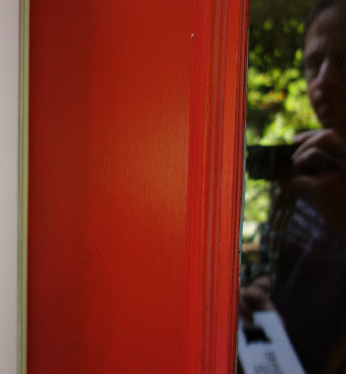
\epsfig{file=figures/color/reddoor.eps,width=1.3in}
%
\epsfig{file=figures/color/reddoorspec.eps,width=1.6in}
%}}
%\sublabel{c}{\centerline{
%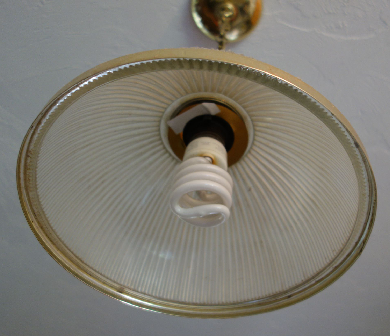
\epsfig{file=figures/color/fourlamp.eps,width=1.7in}
%
\epsfig{file=figures/color/neon.eps,width=1.5in}}}
\caption{The light spectra from some everyday objects, analyzed by the spectrograph of
  \fig{\ref{fig:colorWavelengths}}.  (a) A leaf, with some
  yellowish highlights, shows primarily green, with a little red (red
  and green can combine to appear yellow).  (b) A
  red door.  (c)  A fluorescent light (when turned on) shows the discrete spectral wavelengths at
  which the gas fluoresces.
}
\label{fig:examples1}
\end{figure} 


\subsection{Light Power Spectra}

The light intensity at each wavelength is called the {\bf power spectrum} of the
light.  The color appearance of light is determined by many factors, including the image context in which the light is viewed; but a very important factor in determining color appearance is the power spectrum. In this initial discussion of color, we will assume that the power spectrum of light determines its appearance, although you should remember that this is true only within a fixed visual context.

\marginnote{Why does the sky look blue? And why does it look orange during a sunset? 
\\[6pt]
\centerline{
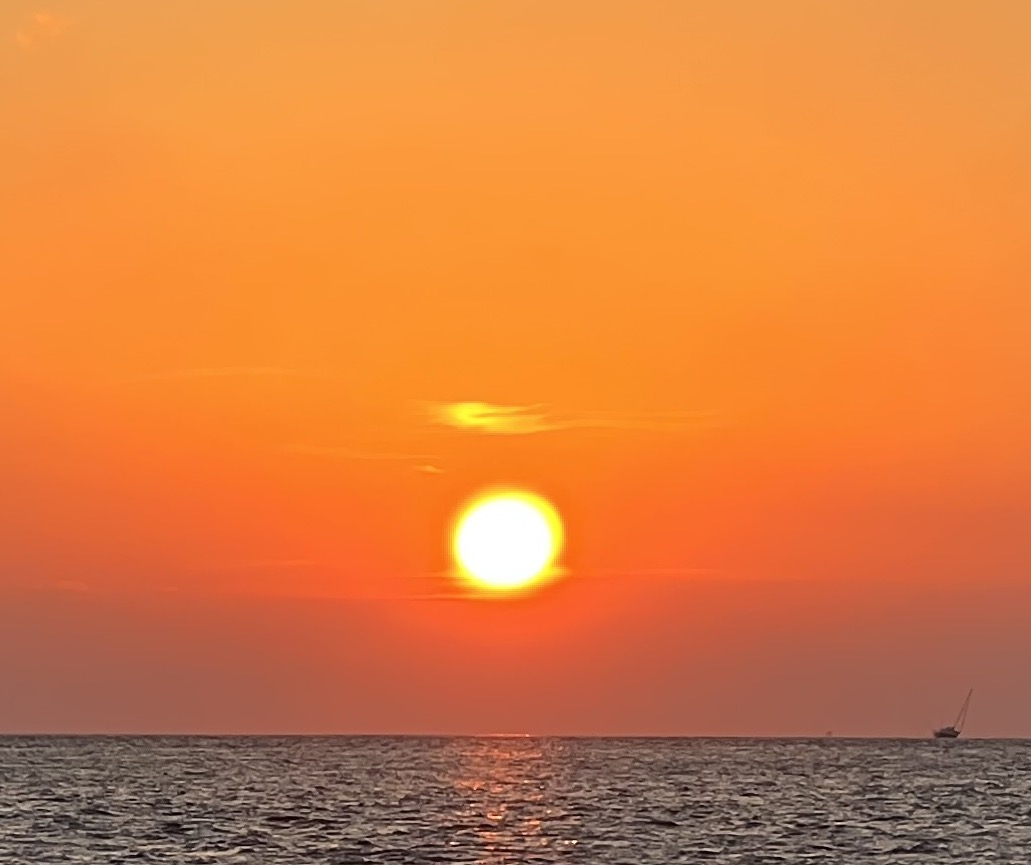
\includegraphics[width=.4\linewidth]{figures/color/sunset_key_west.jpg}
}
}[-1.6in]

\Fig{\ref{fig:examples1}} shows a spectrograph visualization of some light power spectra (the right image of each row) along with the image that the spectrograph was pointed toward (left images).
\Fig{\ref{fig:sources}} shows the spectrum of a blue sky, plotted as 
intensity as a function of wavelength.



\begin{figure}
\centerline{
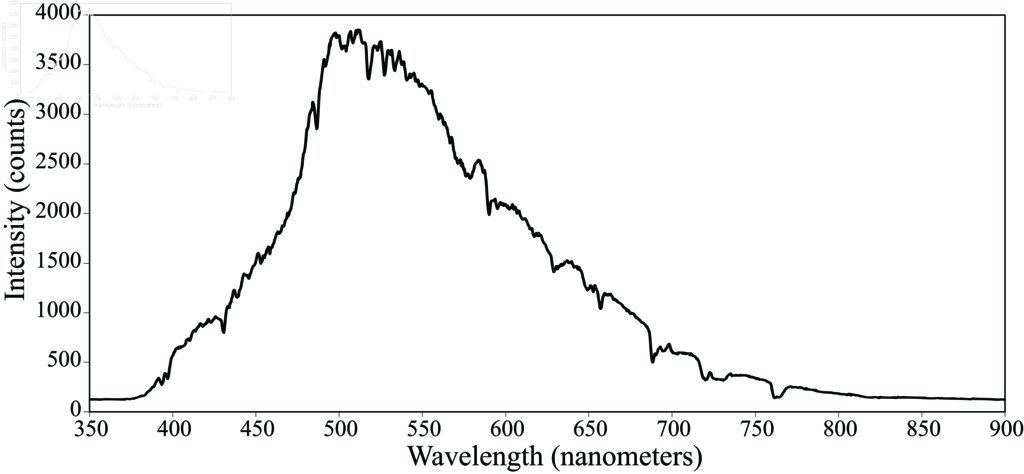
\includegraphics[width=0.7\linewidth]{figures/color/Spectrum_of_blue_sky.eps}
%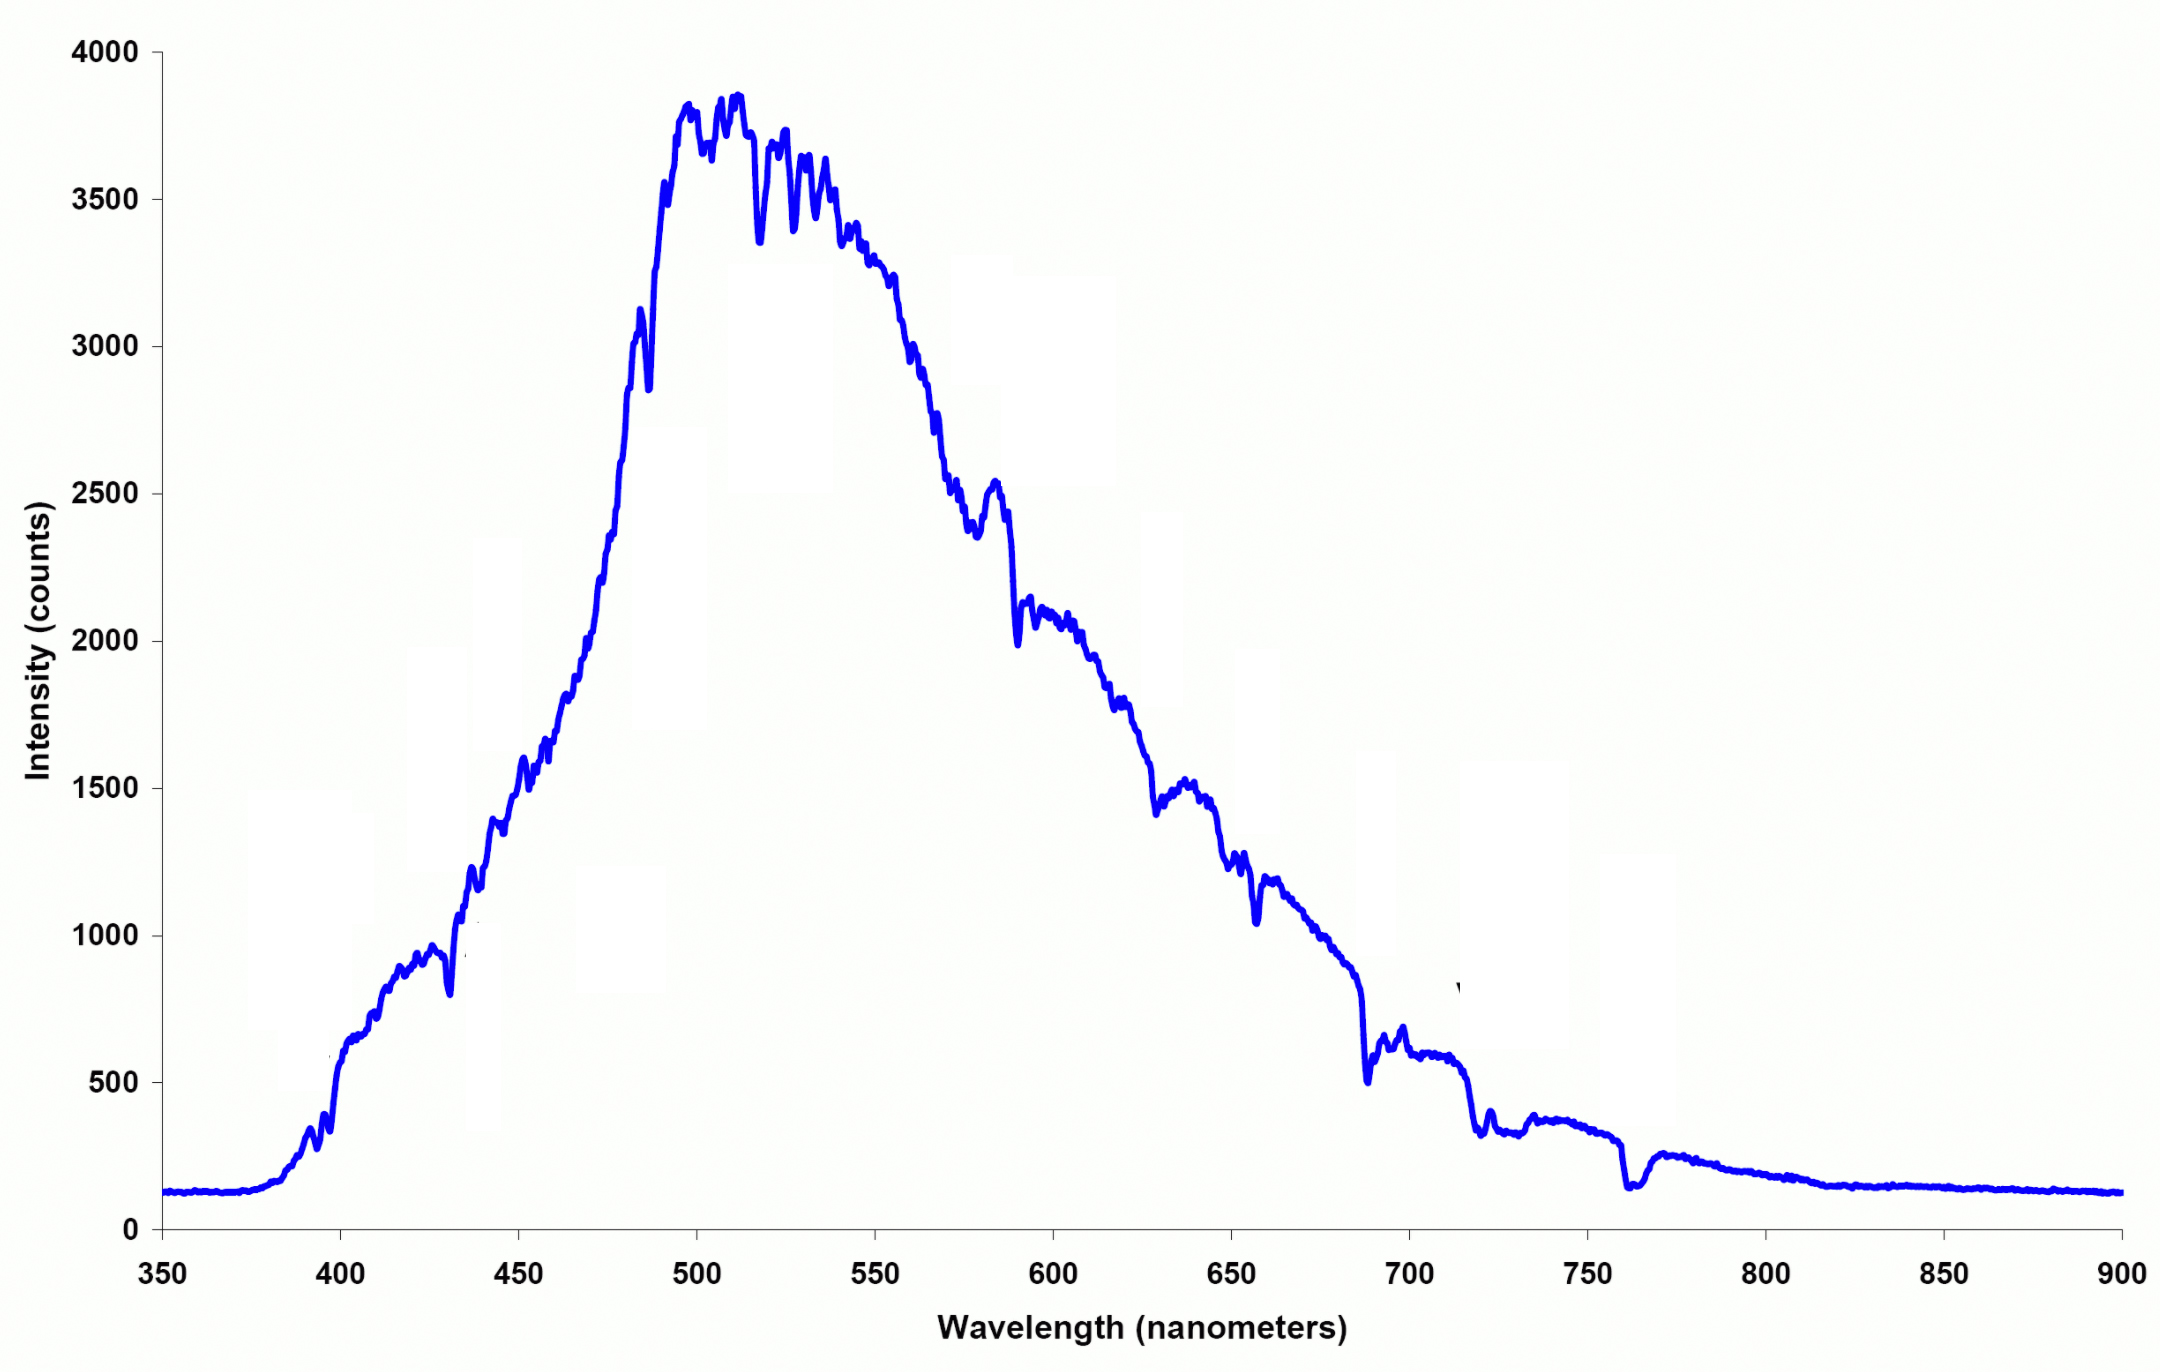
\epsfig{file=figures/color/blueSky.jpg,width=3in}
~~~~~

\includegraphics[width=.15\linewidth]{figures/color/IMG_0122.jpg}
}
\caption{Power spectrum of blue skylight \cite{blueskyWiki}.}
\label{fig:sources}
\end{figure}


\subsection{The Color Appearance of Different Spectral Bands}

It is helpful to develop a feel for the approximate color appearance of different
light spectra.  Again, we say the approximate appearance because the subjective appearance can change according to other factors than just the spectrum.

The visible spectrum lies roughly in the range between 400 and 700 nm,
see \fig{\ref{fig:rainbow}}.  We can divide the visible spectrum into
three 100 nm bands, and study the appearance of light power
spectra where power is present or absent from each of those three
bands, in all of the eight ($2^3$) possible combinations.


\begin{figure}
\centerline{
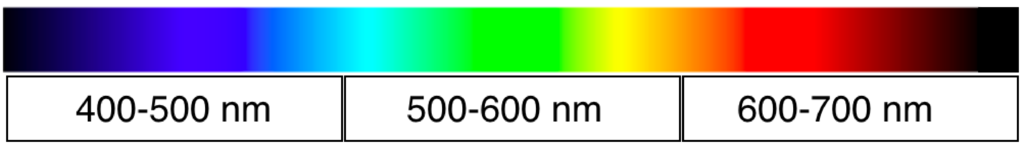
\epsfig{file=figures/color/rainbow3.eps,width=5in}}
\caption{The approximate color appearance of light over different
  spectral regions.}
\label{fig:rainbow}
\end{figure}

Light with spectral power distributed in just the 400--500 nm
wavelength band will look some shade of blue, the exact hue depending
on the precise distribution.  Light in the 500--600 nm band will
appear greenish.  Most distributions within the 600--700 nm band will
look red.

White light is a mixture of all spectral colors.  A spectrum of light
containing power evenly distributed over 400---700 nm would appear approximately
white.  Light with no power in any of those three bands, that is, 
darkness, appears black.

There are three other spectral classes left in this simplified grouping
of spectra:  spectral power present in two of the spectral
bands, but missing in the third.
Cyan is a combination of both blue and green, or roughly spectral
power between 400 and 600 nm.  In printing and color film
applications, this is sometimes called {\em minus red}, since it is the
spectrum of white light, minus the spectrum of red light.  The blue
and red color blocks, or light in the 400--500 nm band, and in the
600--700 nm band, is called magenta, or minus green.  Red and green together,
with spectral power from 500--700 nm, make yellow, or minus blue (\fig{\ref{fig:names}}). 

\begin{figure}
\centerline{
\includegraphics[width=1.0\linewidth]{figures/color/cartoonColor2.eps}
}
%\epsfig{file=figures/color/cartoonColor2.eps,width=5in}}
\caption{For coarse orientation only, this cartoon model gives the color appearance of different spectral bands of the spectrum of visible light.}
\label{fig:names}
\end{figure}



\subsection{Light Reflecting from Surfaces}

When light reflects off a surface, the power spectrum alters in ways that depend on the surface’s characteristics and geometry. These
changes in light allow us to perceive objects and surfaces by observing their influence on the reflected light.

The interaction between light and a surface can be quite complex. Reflections can be specular or diffuse, and the reflected
power spectrum may depend on the relative orientations of the incident
light, surface, and the observed reflected ray. In its full generality, the reflection of light from a surface is described by the
bidirectional reflectance distribution function (BRDF) \cite{Nicodemus1965,Matusik2002}.
For this discussion, we will focus on diffuse
surface reflections, where the power spectrum of the reflected light, $r(\lambda)$,
is proportional to the wavelength-by-wavelength product of the power
spectrum of the incident light, $\imgin (\lambda)$, and a {\bf reflectance
  spectrum}, $s(\lambda)$, of the surface:
\begin{equation}
r(\lambda) = k \imgin (\lambda) s(\lambda),
\end{equation}
where the proportionality constant $k$ depends on the reflection geometry.
This diffuse reflection model characterizes
most matte reflections.  Such wavelength-by-wavelength scaling
is also a good model for the spectral changes to light caused by transmission
through an attenuating filter.  The incident power spectrum is
then multiplied at each wavelength by the {\bf transmittance spectrum} of
the attenuating filter.

Some reflectance spectra of real-world surfaces are plotted in
\fig{\ref{fig:sourcerefl}}.  The flower {\em Hepatica Nobilis} (solid line) is blue, while {\em Pyrostegia venusta} (dotted line) is orange.

\begin{figure}[t]
\centerline{
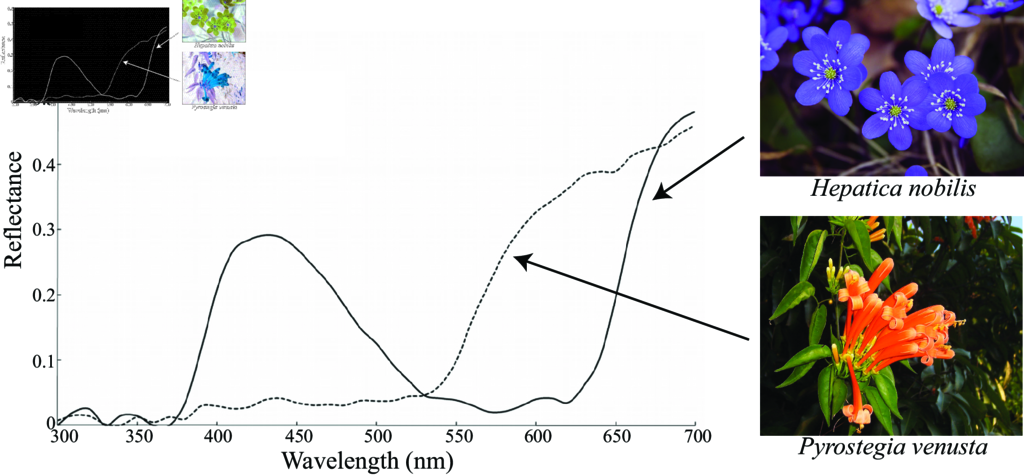
\includegraphics[width=1.0\linewidth]{figures/color/flowerSpectra.eps}
}
%\centerline{
%\sublabelnp{(a) reflectance functions of two flowers}{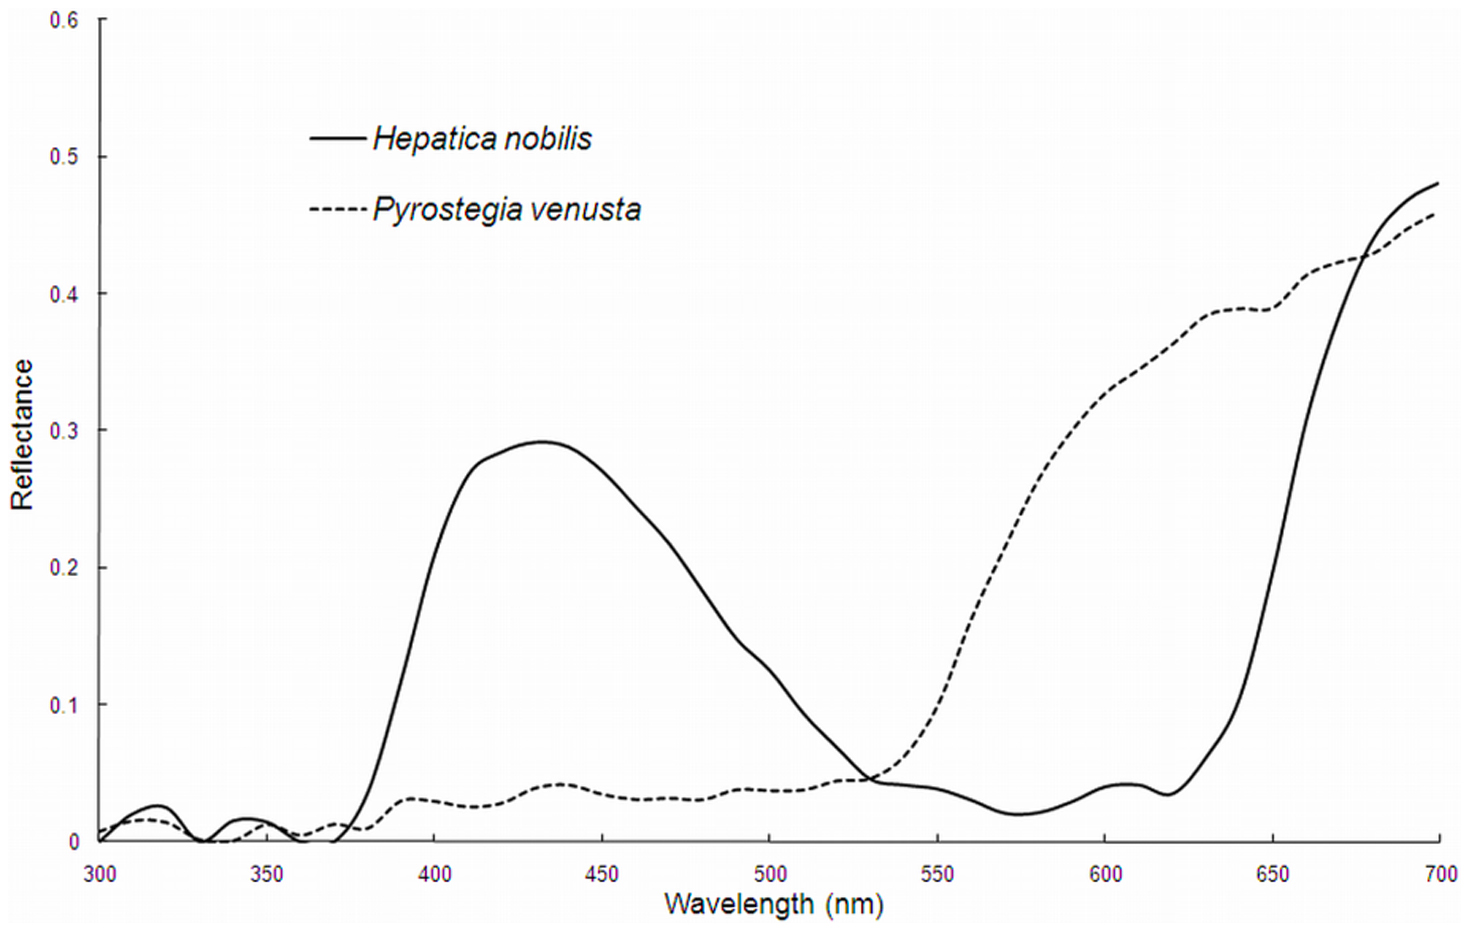
\epsfig{file=figures/color/flowerSpectra.jpg,width=3in}}
%\sublabelnp{(b) Hepatica nobilis (solid line)}{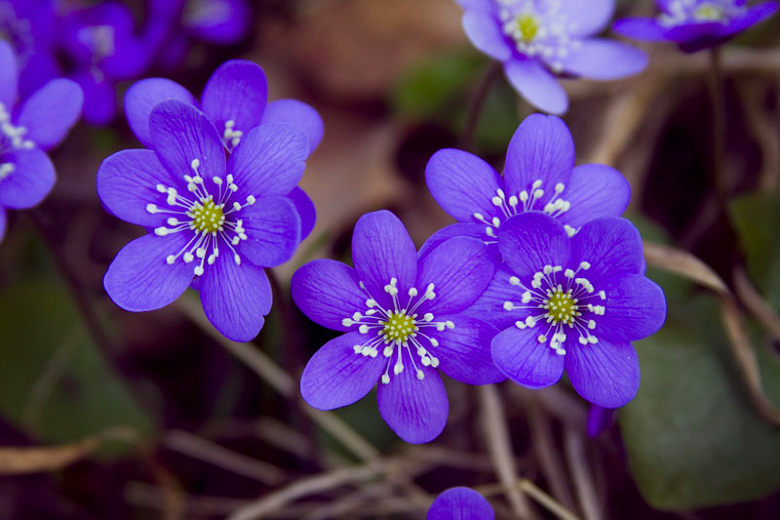
\epsfig{file=figures/color/nobilis.jpg,width=1.3in}}
%\sublabelnp{(c) Pyrostegia venusta (dotted line)}{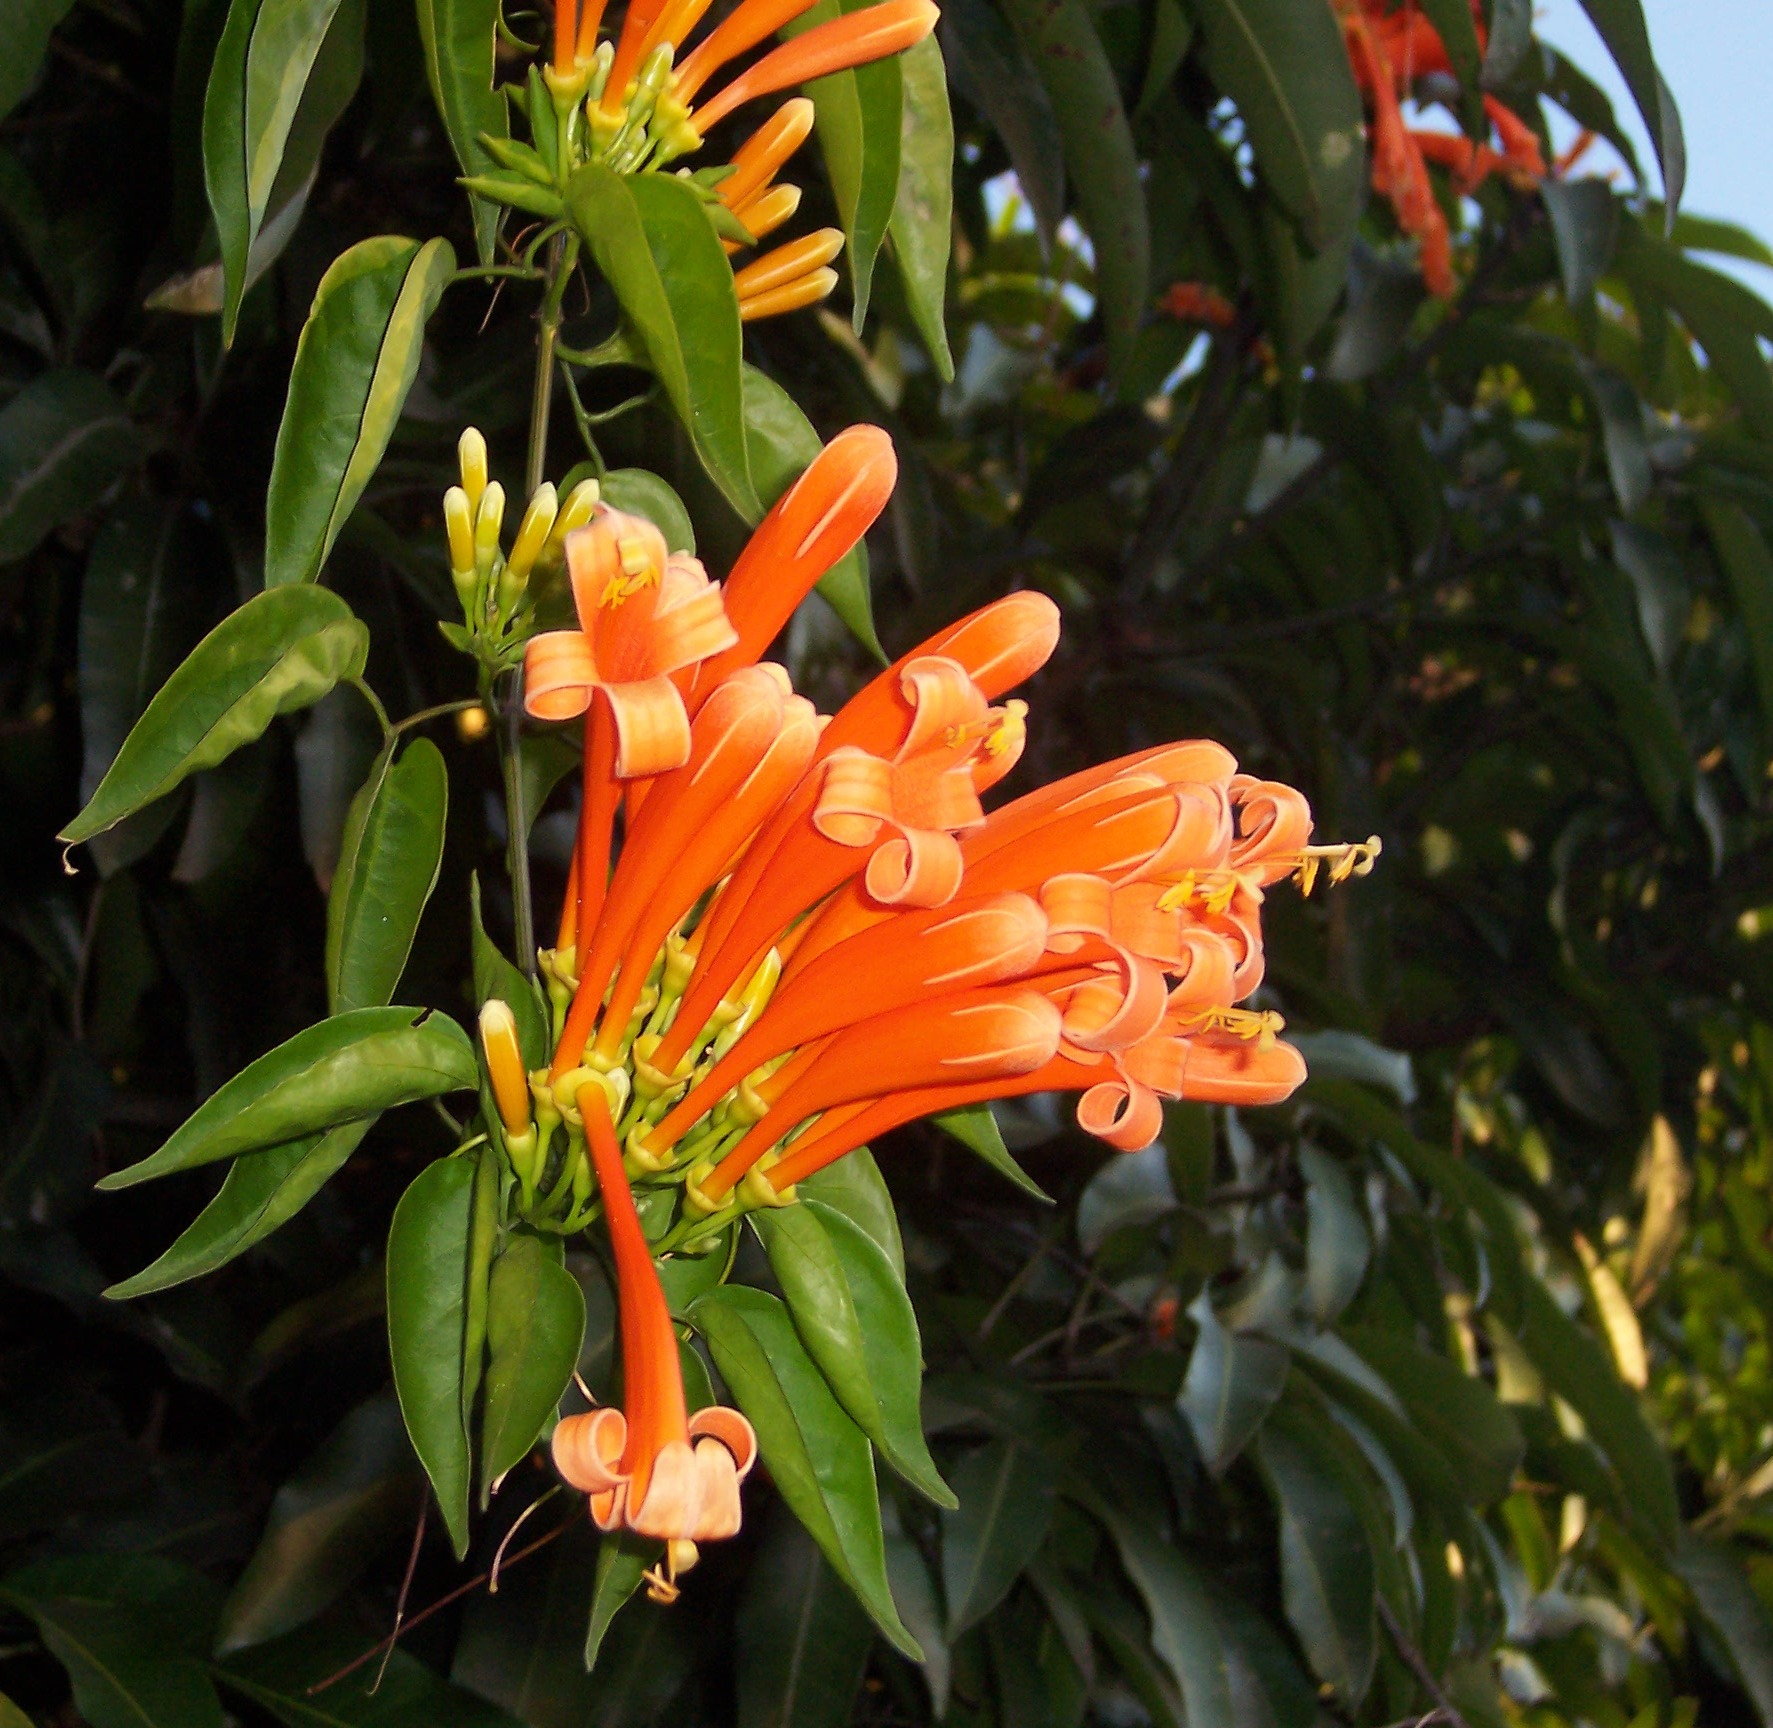
\epsfig{file=figures/color/Pyrostegia_venusta3.jpg,width=1.3in}}
%}
\caption{Reflectance spectra from two flowers \cite{Arnold2010}. The blue {\em Hepatica nobilis} flower \cite{nobilis} and the orange flower, {\em Pyrostegia venusta} \cite{venusta}.}
\label{fig:sourcerefl}
\end{figure}




The reflectance spectrum of a surface often carries valuable information about the material being viewed, such as whether a fruit is ripe, whether a human's skin is healthy, or whether the material differs from another viewed material.  It may be the case that a low-dimensional version of the surface reflectance spectrum is sufficient for many visual tasks, and as we see subsequently, the human visual system represents color with only three numbers.  So it is an important visual task to estimate either the surface reflectance spectrum, or a low-dimensional summary of it. 


To estimate surface colors by looking, a vision system has the task of estimating the illumination spectrum and the surface reflectance spectra, from observations of only their products.
When the illumination is white light with equal power in all spectral bands,
the observed reflected spectrum is proportional to the reflectance spectrum of the
material itself.  However, under the more general condition of unknown illumination color, a visual system will need to estimate the surface reflectance spectrum, or projections of it, by taking the context of nearby image information into account.

There are many proposed algorithms to do that, ranging from heuristics, for example, assuming the color of the brightest observed object is white \cite{McCann76}, to statistical methods \cite{Brainard97} and neural network based approaches \cite{Barron2015}.
Even humans don't solve the problem perfectly or consistently, revealed especially through the internet meme of \#TheDress \cite{Bleasdale2015}, 
%``TheDress'', 
shown in \fig{\ref{fig:thedress}}.  


\begin{figure}[t]
\centerline{
%\sublabel{a}{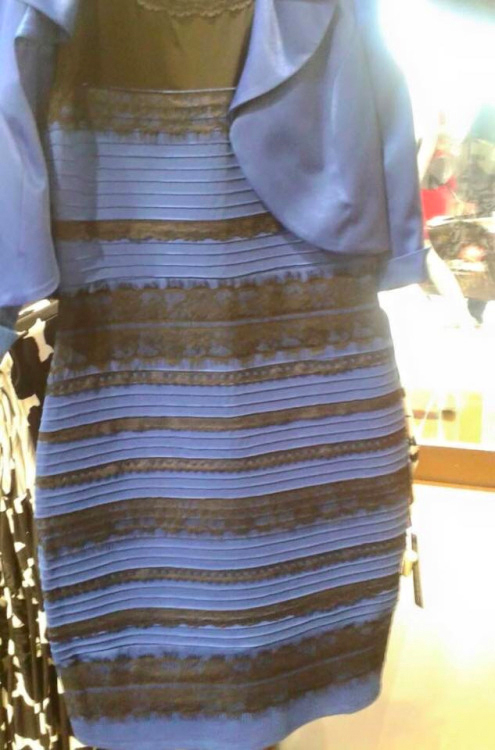
\epsfig{file=figures/color/thephotoofthedress.jpg, width=1.9in}}
%\sublabel{b}{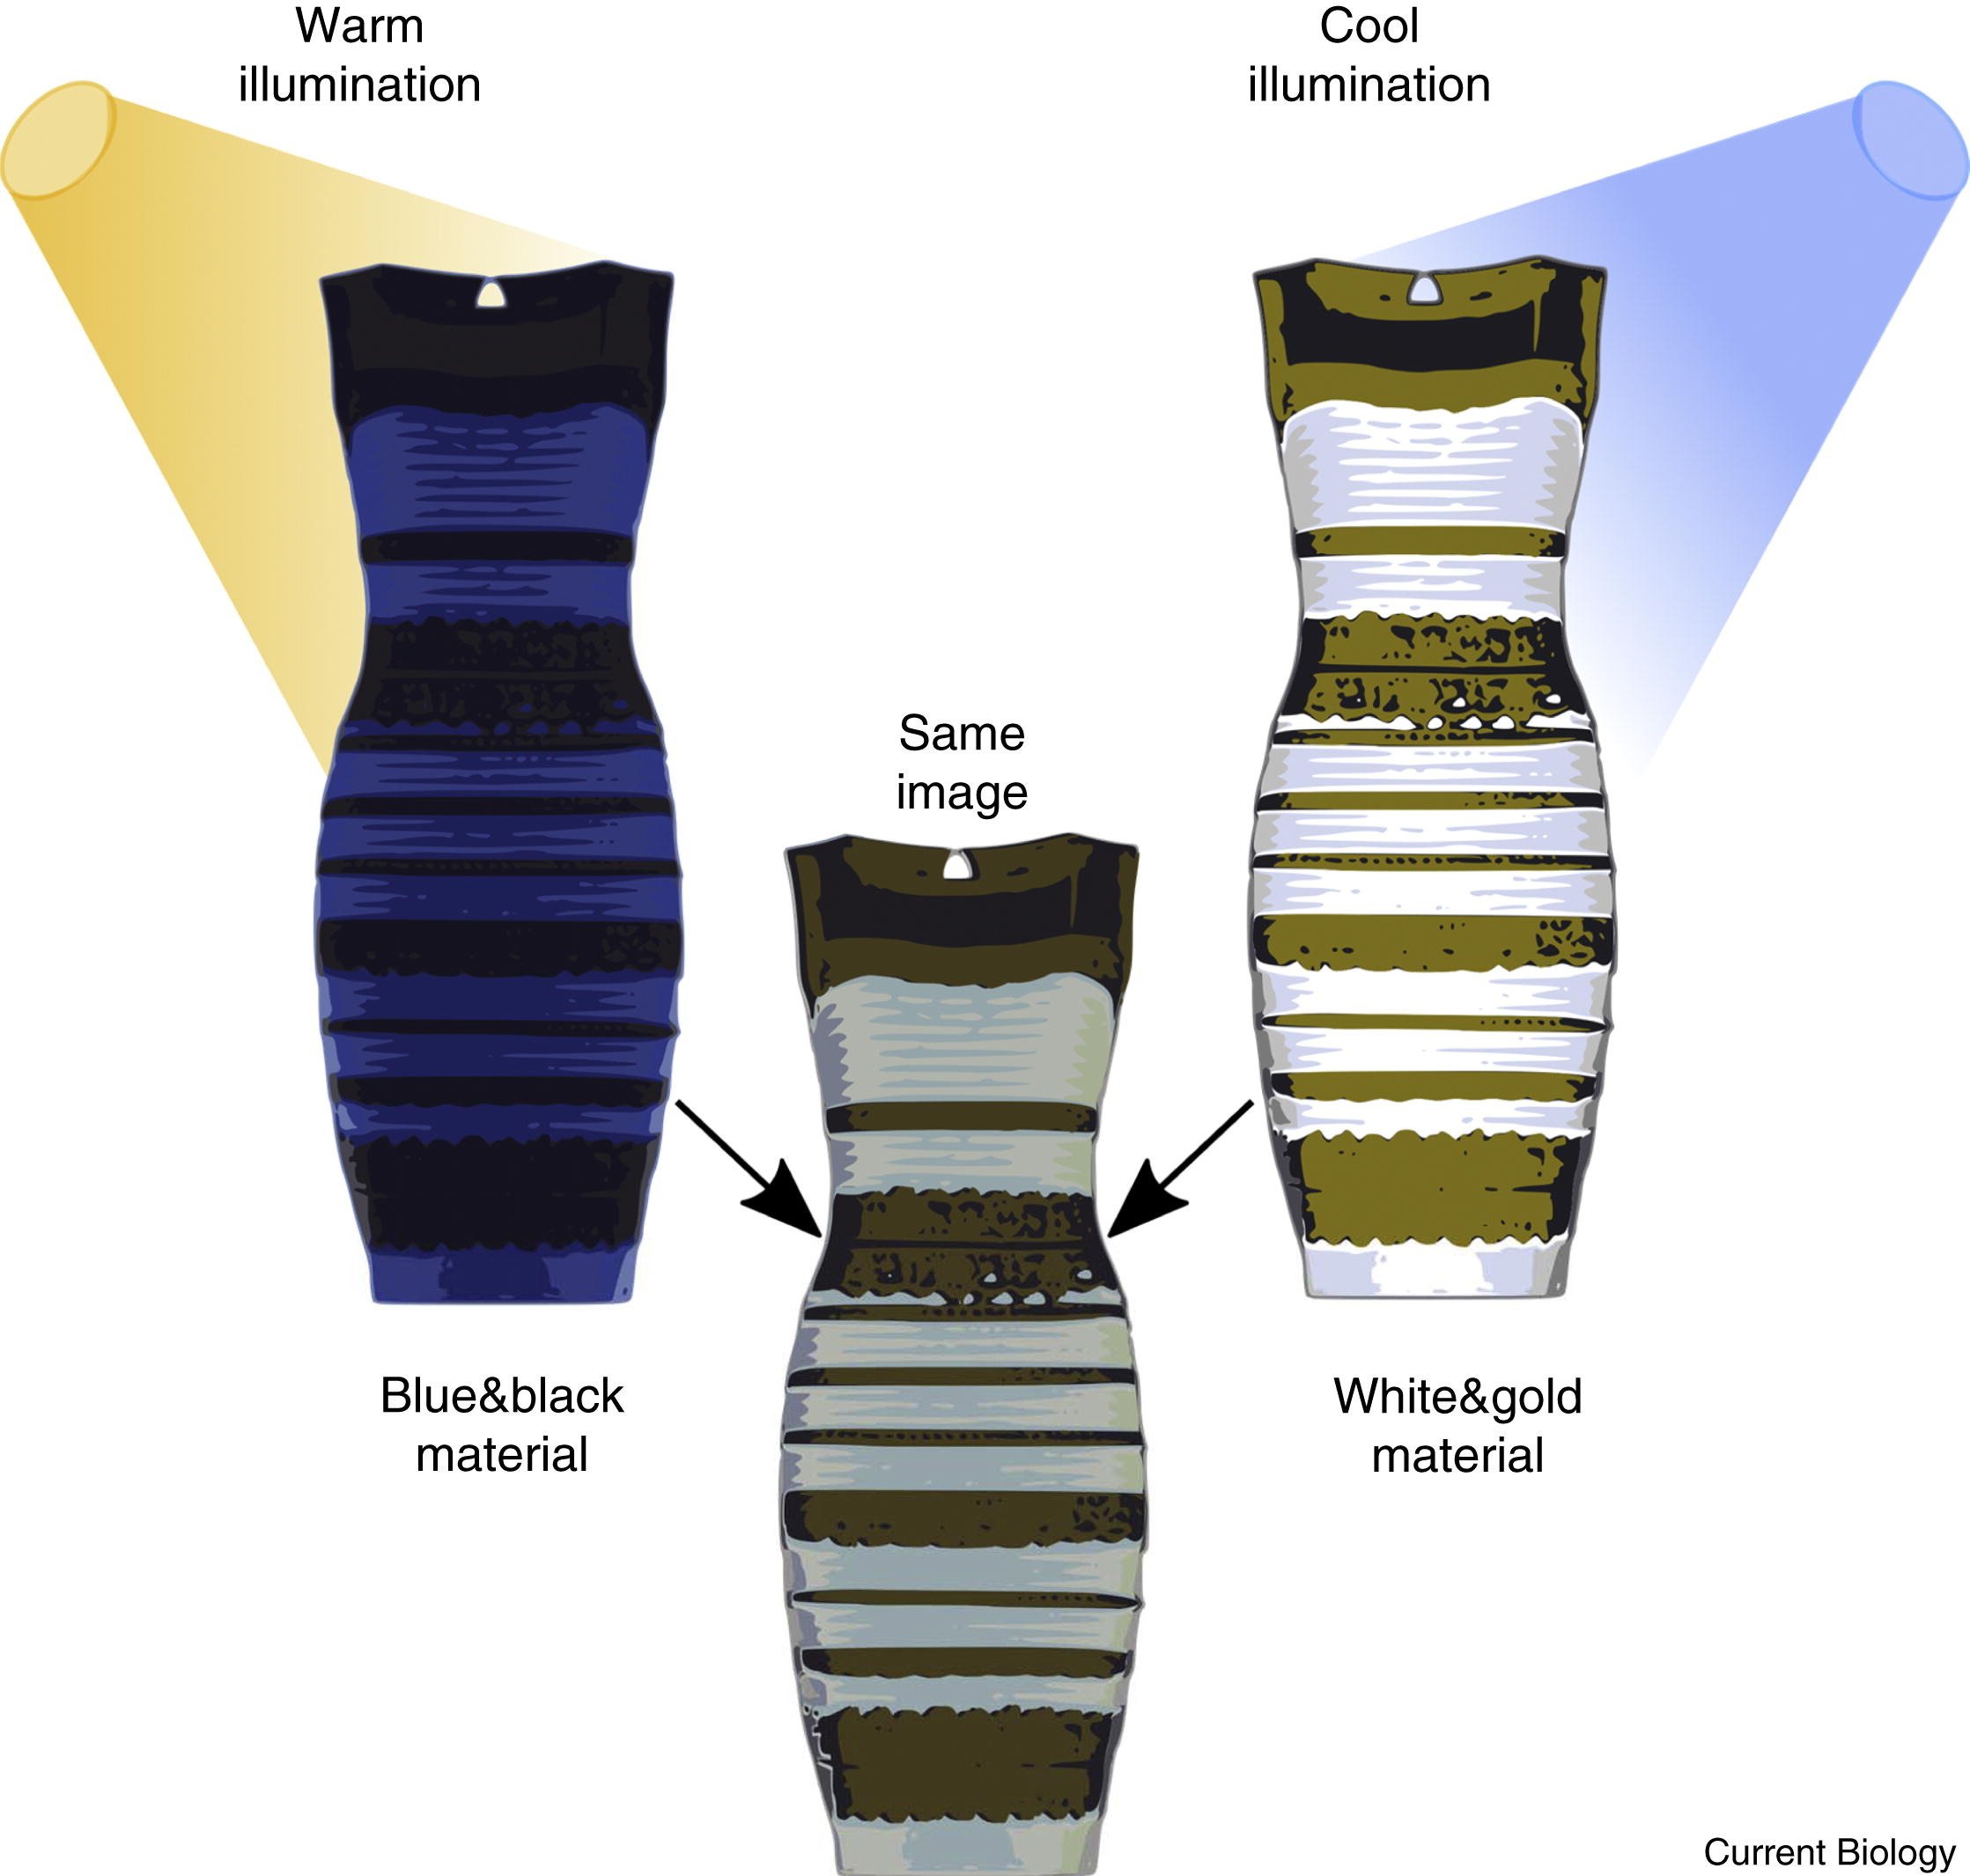
\epsfig{file=figures/color/gr2_lrg.jpg, width=2.9in}}
\sublabel{a}{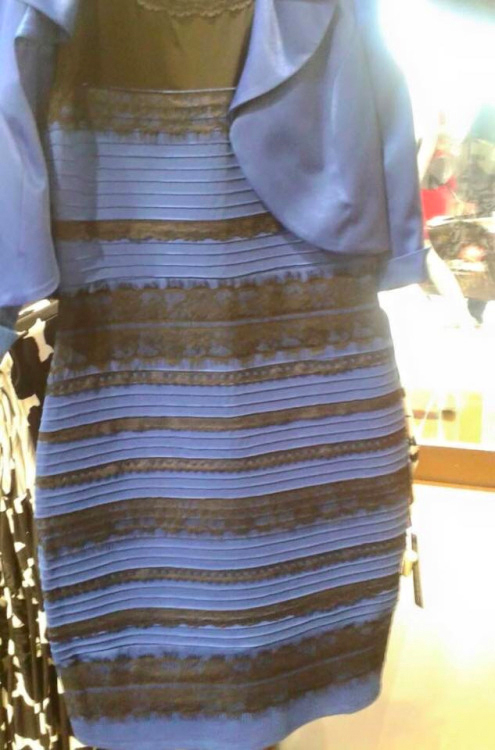
\includegraphics[width=1.9in]{figures/color/thephotoofthedress.jpg}}
\sublabel{a}{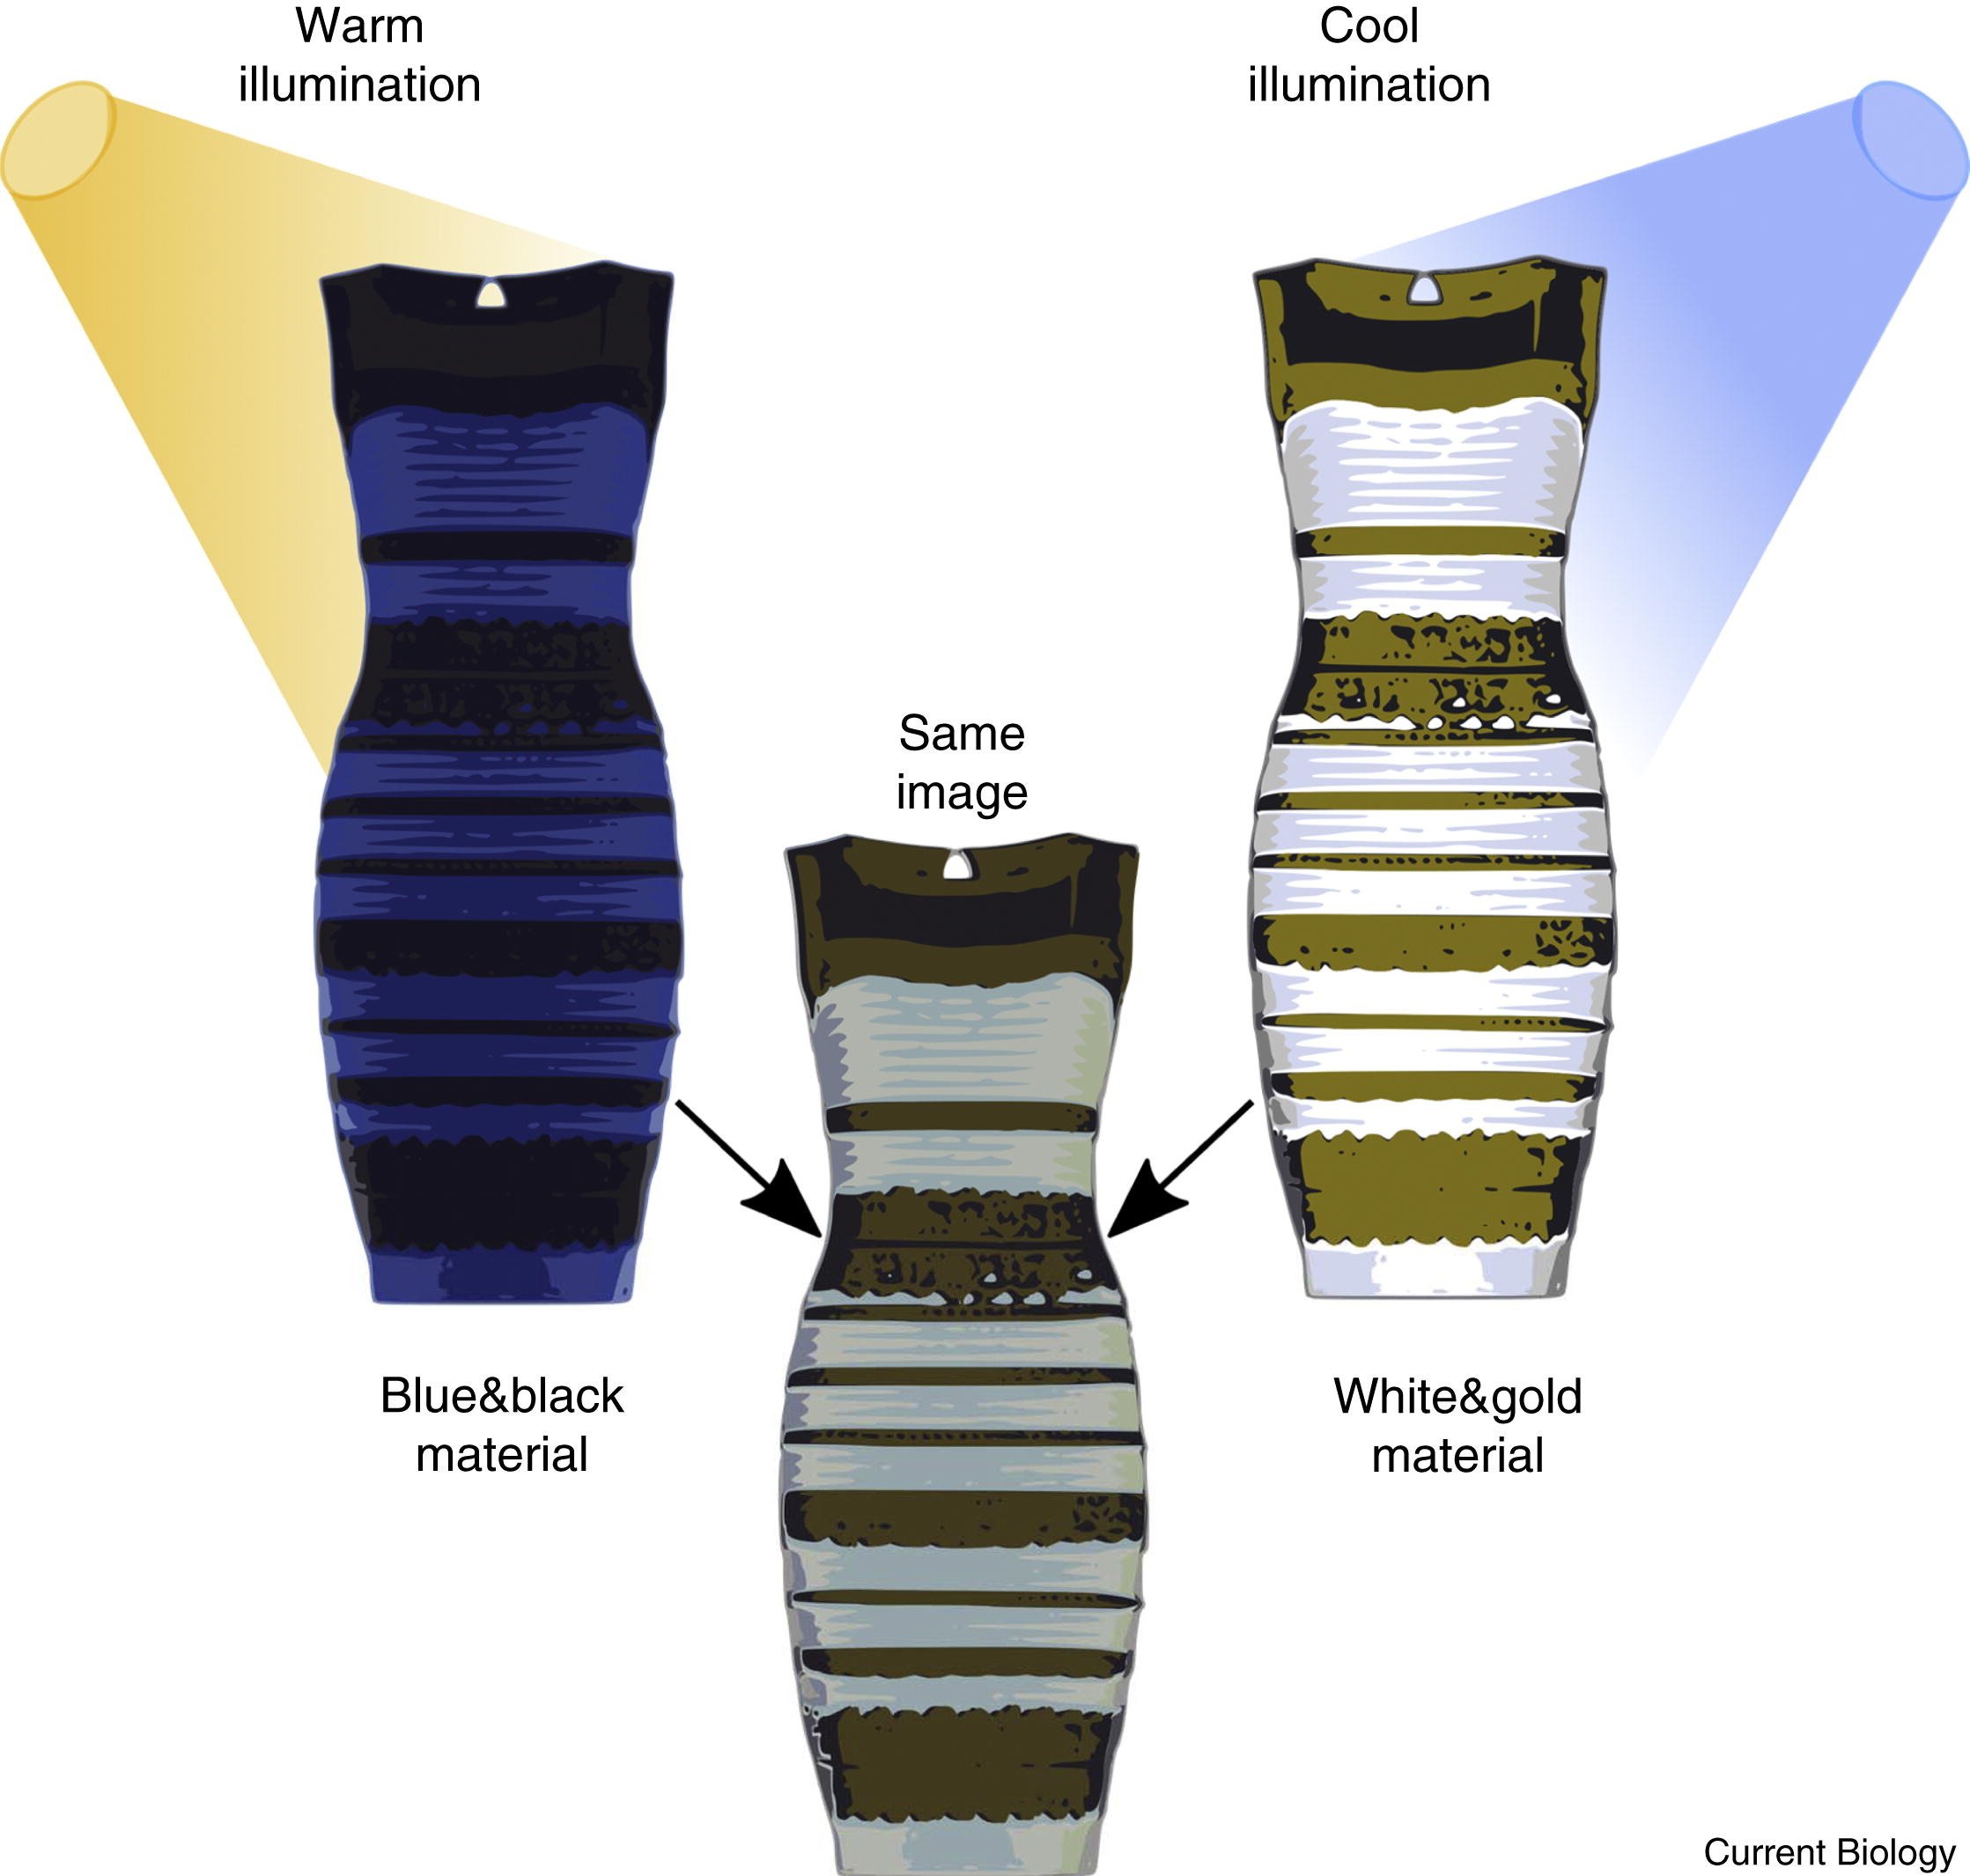
\includegraphics[width=2.9in]{figures/color/gr2_lrg.jpg}}
}
\caption{(a) \#The Dress, photographed and posted by \cite{Bleasdale2015}, reprinted with permission.  (b) The spectra of the light we see is the product of an assumed illumination spectrum and the inferred surface reflectance spectra.  If people make different assumptions about the illumination, they can perceive different colors within the same image, as shown in this illustration \cite{Brainard2015}.  Reprinted with permission from Elsevier.
}
\label{fig:thedress}
\end{figure}



The perceived colors of the dress depend on the assumed color of the illumination, and people can disagree significantly about the colors they see \cite{Brainard2015}.  The assumption of a warm, yellowish, illumination color leads to a perception of blue and black material.  The assumption of a cool, blueish illumination leads to a perception of white and gold material.  Both perceptions are consistent with the observed product of illumination and reflectance  seen in the dress image.  

\marginnote{Did you perceive the dress, \fig{\ref{fig:thedress}}, to be black on blue, or gold on white?  Can you make the perception change?}

While such context-dependent effects are important in color perception, as we quantify color perception we will assume that our perception of color depends only on the spectrum of light entering the eye.  This will serve us well for many industrial applications.


\section{Color Perception}

Now we turn to our perception of color.  We first describe the
machinery of the eye, then describe some methods to measure color appearance.  These methods to measure color appearance implicitly assume a white illumination spectrum, but they often serve the needs of industry and science.


\subsection{The Machinery of the Eye}

%Figure~\ref{fig:ramon}~a is a drawing \cite{cajal1904} of the photoreceptors, called the rod and cones, in the retina of the eye.  The tall receptors are the rods, used in low-light levels, and the short ones are the cones, used in color vision.  Interestingly, the light enters from the bottom of the drawing, passing through the nerve fibers and blood vessels before reaching the photosensitive detectors at the top of the image. 



An instrument such as a spectrograph (\fig{\ref{fig:colorWavelengths}} shows a simple one)
can measure the light power spectrum at hundreds of
different wavelengths within the visible band, yielding hundreds of
numbers to describe the light power spectrum.  Despite this, a useful
description of the visual world can be obtained from a much lower
dimensional description of the light power spectrum.  
\marginnote{The retina contains photoreceptors called the rod and cones. Rods are used in low-light levels, and the cones are used in color vision. In low-light, only the rods operate and our vision becomes black and white.}

The human visual
system analyzes the incident light power spectrum with only three
different classes photoreceptors, called the L, M, and S cones because
they sample at the long, medium, and short wavelengths.  This gives
the human visual system a three-dimensional (3D) description of light, with
each photoreceptor class taking a different weighted average of the
incident light power spectrum.

\Fig{\ref{fig:ramon}}{a} shows 
the spatial sampling pattern, for each of the three cone classes, measured from a subject's eye \cite{Hofer2005}. The L cones are
colored red, the M cones green, and the S cones are colored
blue. Note the hexagonal packing of the cones in the retina, and the
stochastic assignment of L, M, and S cones over space.  Note also the much sparser spatial sampling of the S cones than of either the L or M cones.
\Fig{\ref{fig:ramon}}{b} shows the spectral sensitivity curves
for the L, M, and S cones.  This sampling pattern was measured from near the {\bf fovea}, where there are no rods, and the cones are close-packed.


\begin{figure}[t]
\centerline{
%\sublabel{a}{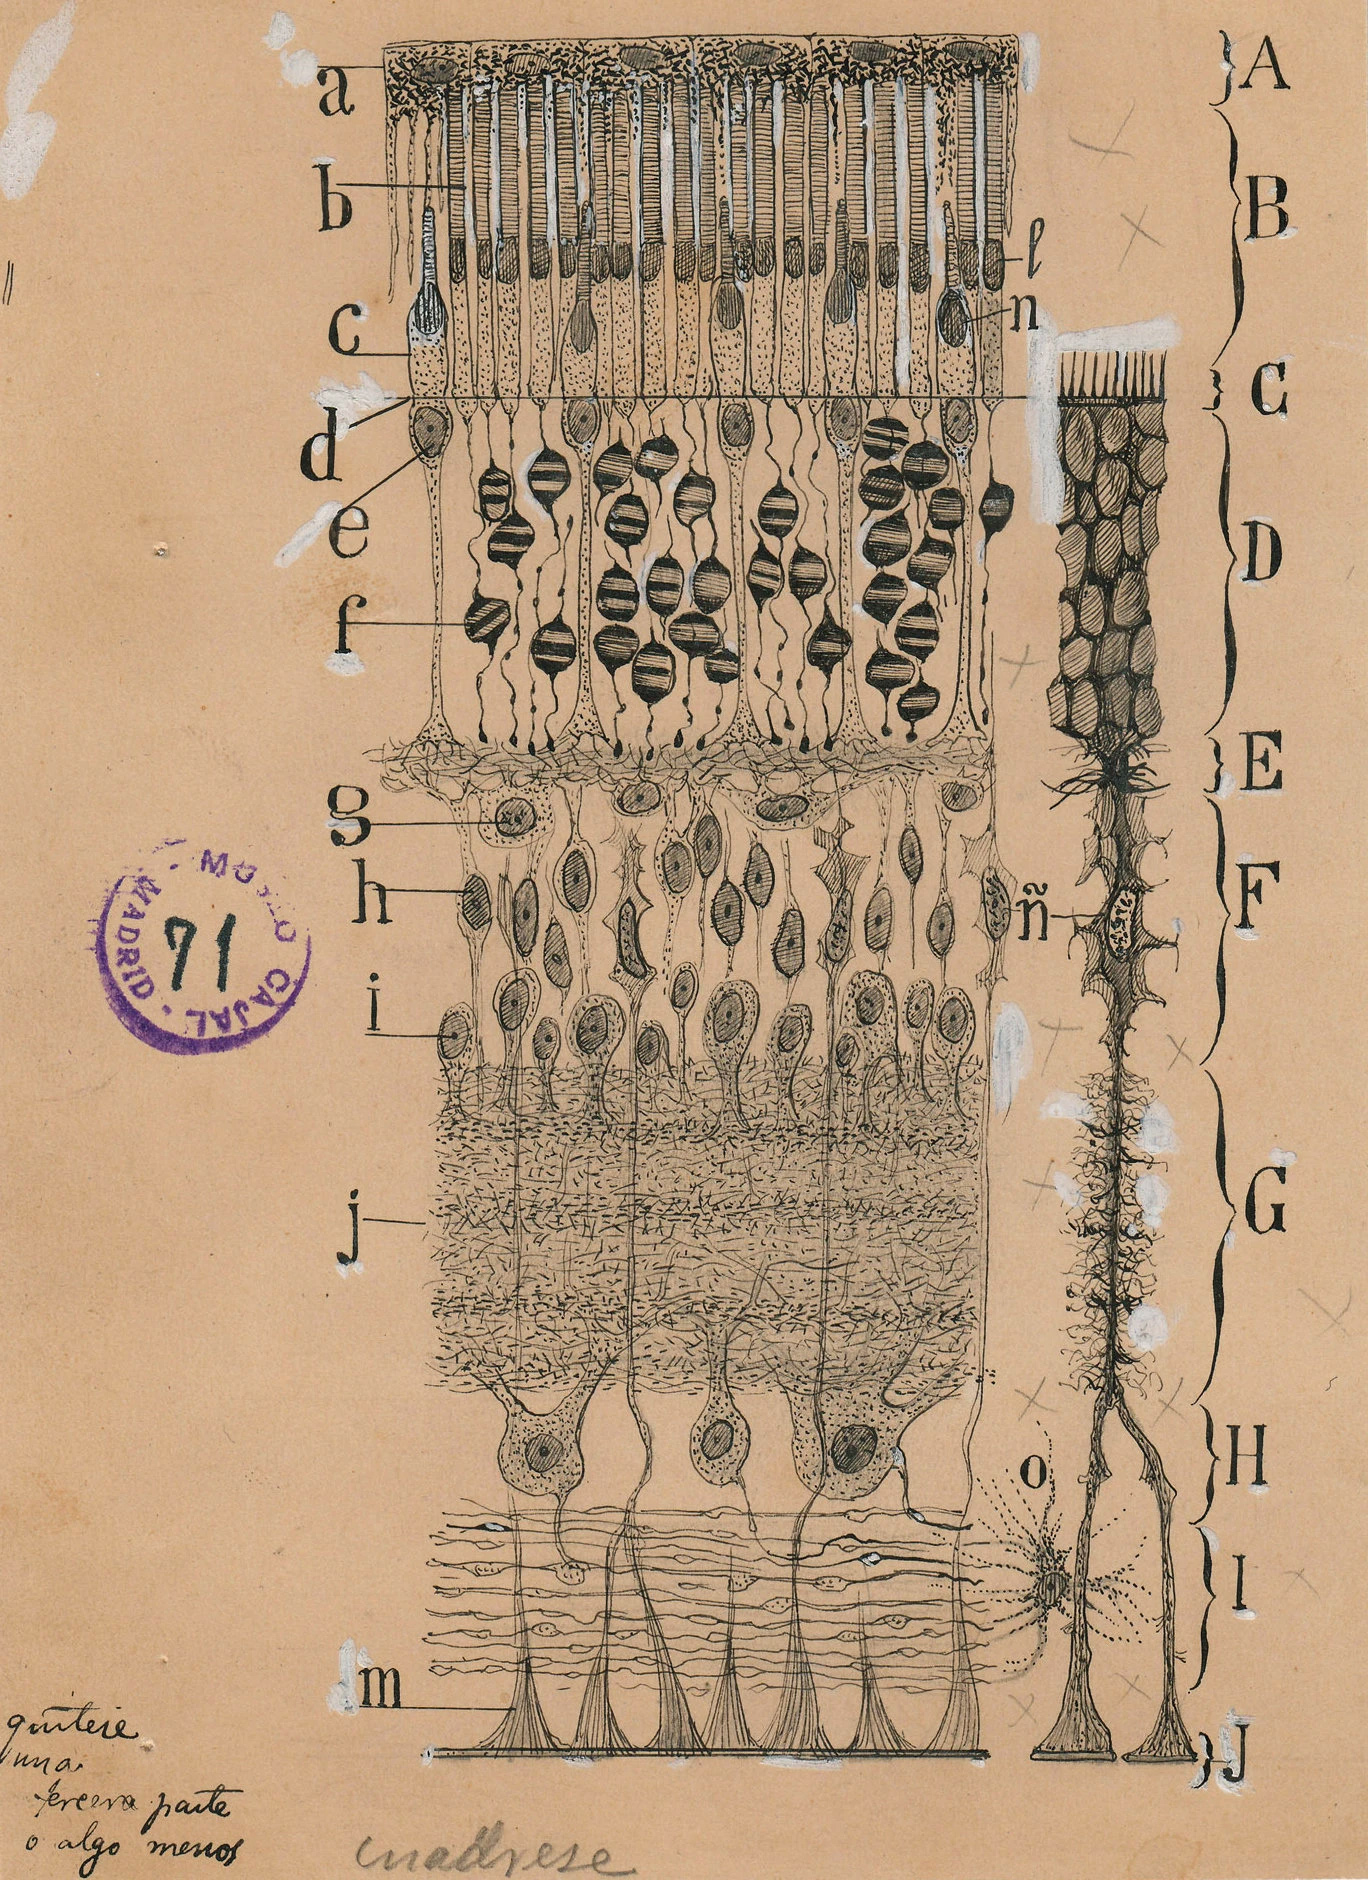
\epsfig{file=figures/color/ramonycajal,width=2in}}
\sublabel{a}{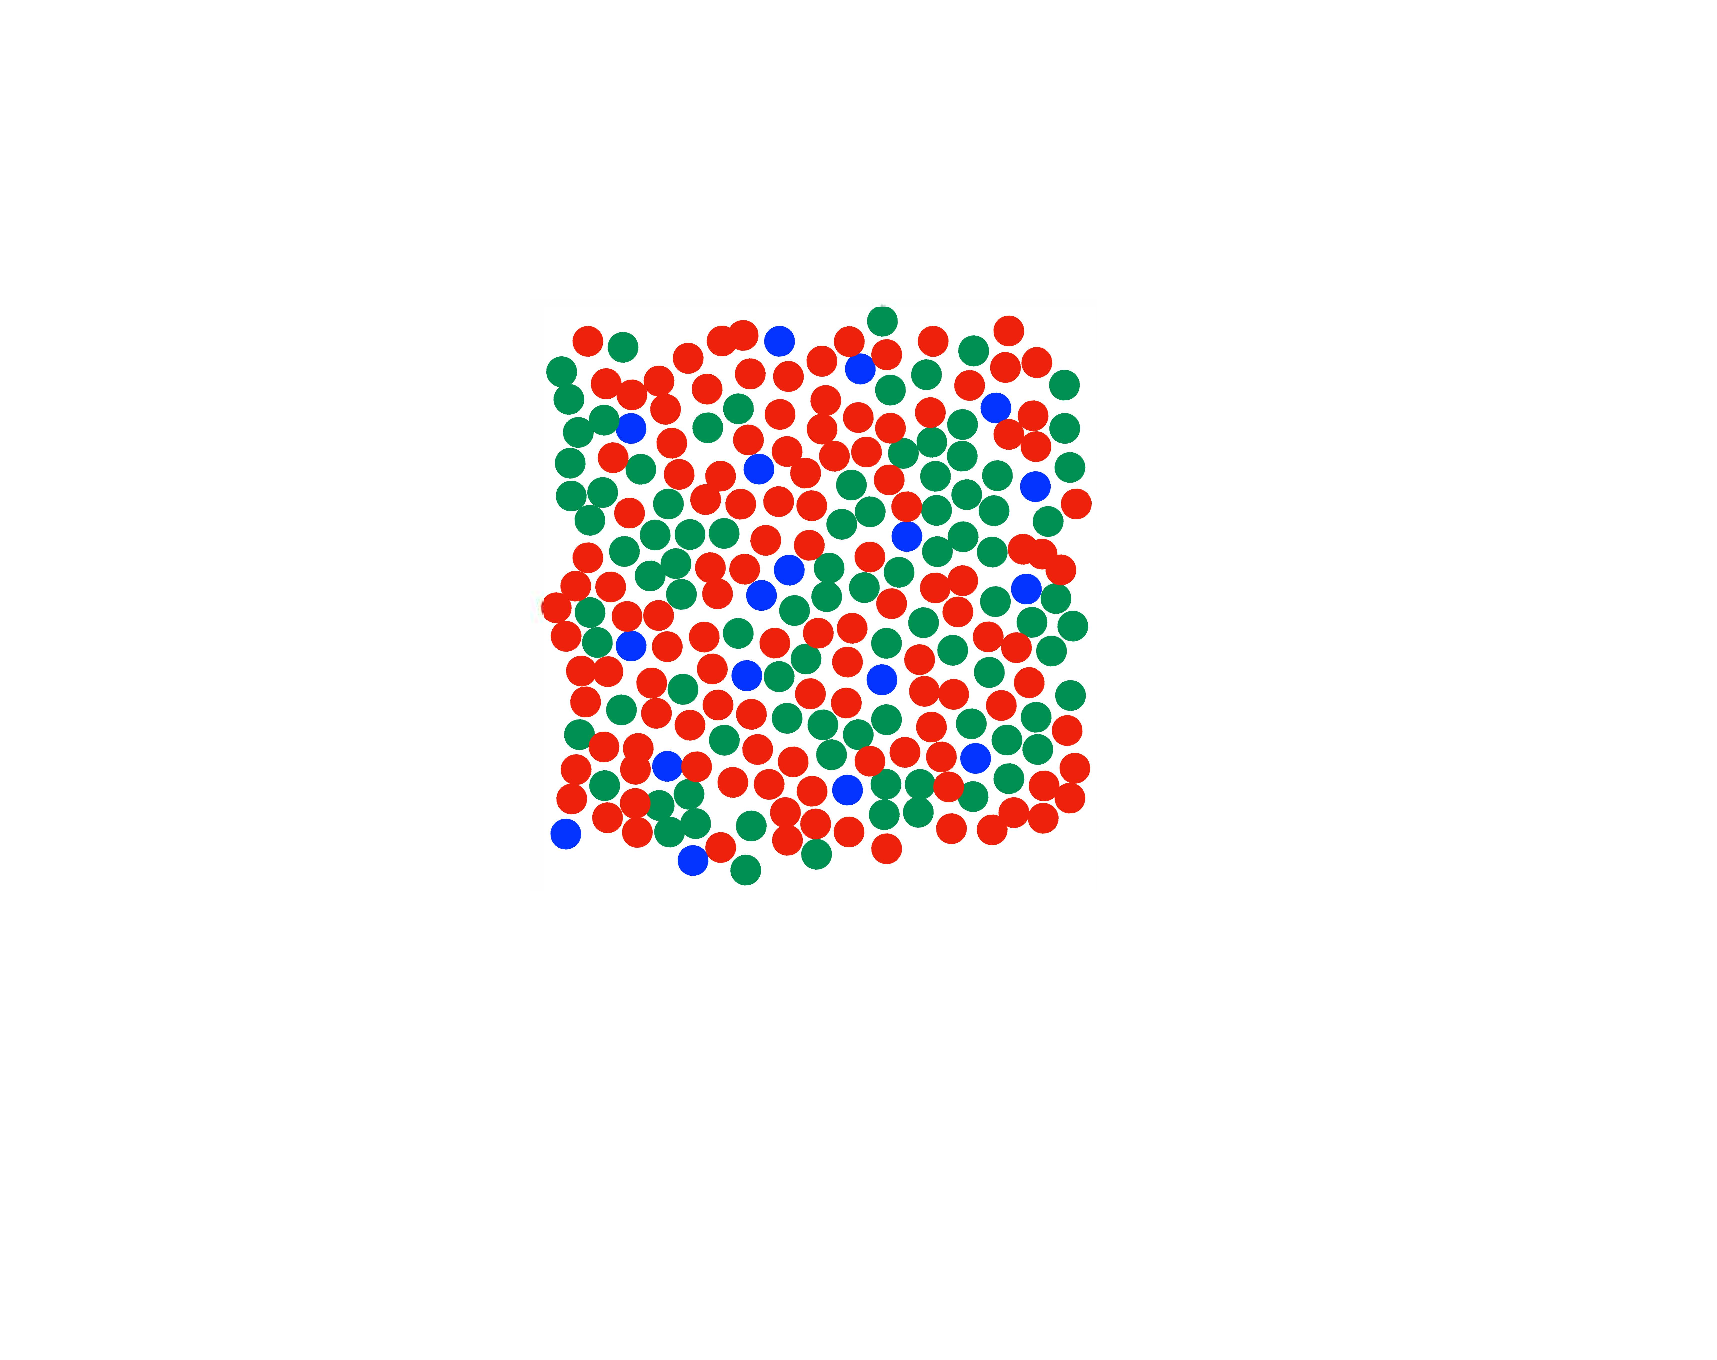
\epsfig{file=figures/color/YYretina.pdf,width=2in}}
\sublabel{b}{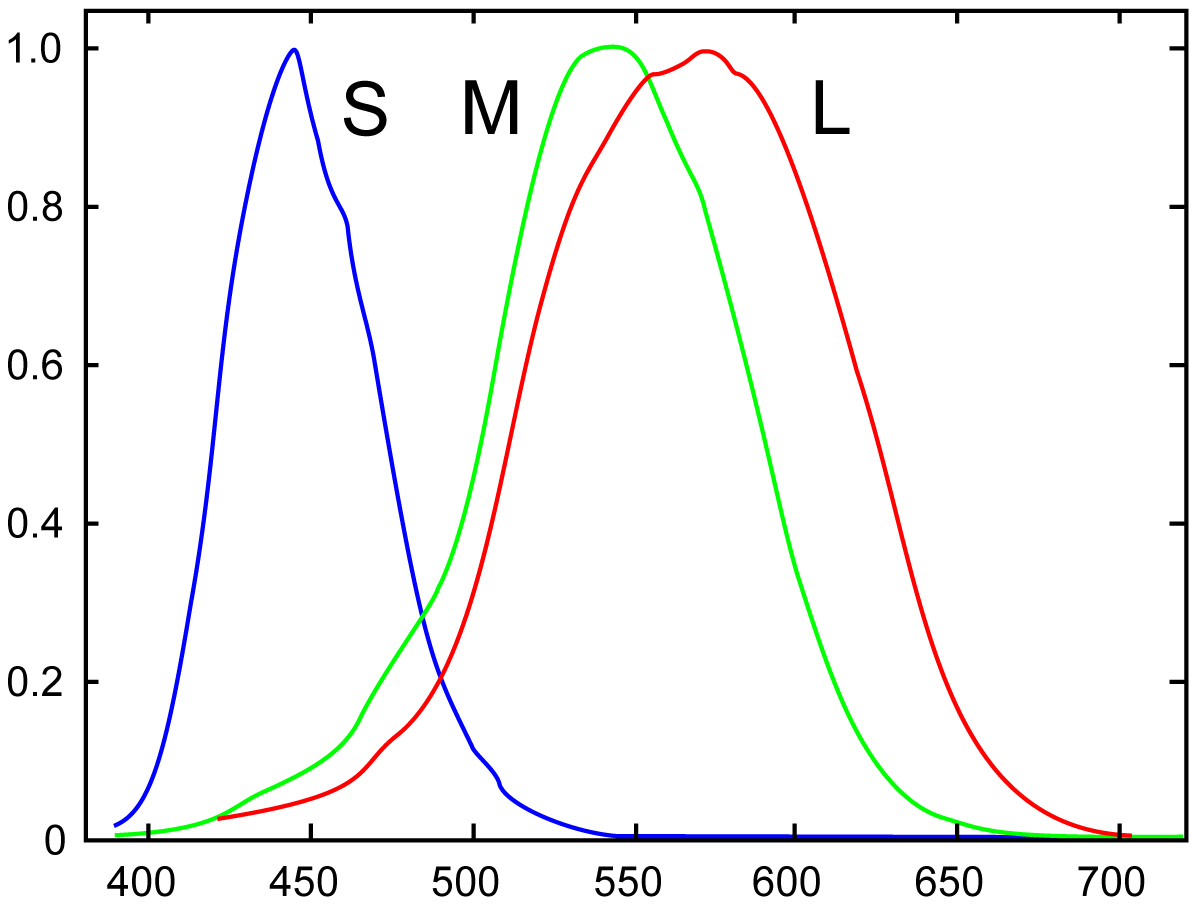
\epsfig{file=figures/color/Cones_SMJ2_E.jpg,width=2.5in}}
}
%\centerline{
%\sublabel{c}{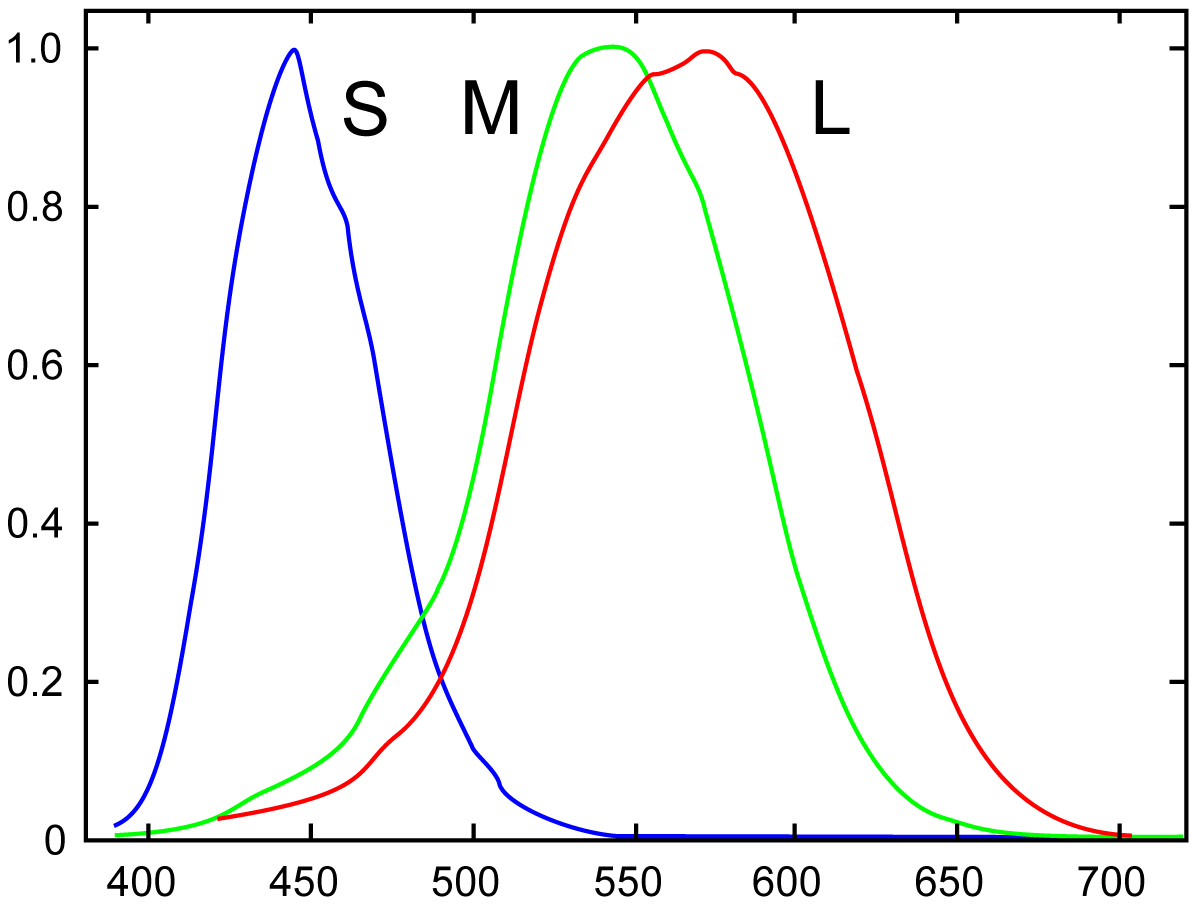
\epsfig{file=figures/color/Cones_SMJ2_E.jpg,width=4in}}
%}
\caption{
%(a) Drawing of the eye's photoreceptors by the physiologist Ramon y Cajal \cite{cajal1904}.
 (a)  Measured cone receptor classes and positions in a human retina, with cone receptor classes shown as red, green, and blue (subject YY, redrawn from \cite{Hofer2005}).
(b) Photoreceptor sensitivities as a function of light wavelength  \cite{Vanessaezekowitz2007}.}
\label{fig:ramon}
\end{figure}


We can describe the photoreceptor responses using matrix algebra.
If the matrix $\mathbf{C}_{\mbox{eye}}$ consists of the spectral sensitivities of the
L, M, and S cones in three rows, and the vector $\mathbf{t}$ is a column
vector of the spectrum of light incident on the eye, then the L, M,
and S cone responses will be the product,
\begin{equation}
    \begin{bmatrix}
    L  \\
    M  \\
    S \\
    \end{bmatrix}
= \mathbf{C}_{\mbox{eye}} \, \mathbf{t}
\label{eq:lmsct}
\end{equation}

The fact that our eyes have three different classes of photoreceptors
has many consequences for color science.  It determines that there are
three primary colors, three color layers in photographic film, and
three colors of dots needed to render color on a display screen.  In
the next section, we describe how to build a color reproduction system that matches the colors seen in the world by a human observer.

%% \billf{Who first discovered trichromaticity, and how?}


\subsection{Color Matching}

Color science tells us how to analyze and reproduce color.
We seek to build image displays so that the output colors match those of
some desired target, and to manufacture items with the same colors over
time.  Much of the color industry revolves around the ability to repeatably control colors.
Colors can be trademarked (Kodak Yellow, IBM Blue) and we have
color standards for foods.  \Fig{\ref{fig:french}} shows French fry color
standards.

\begin{figure}[t]
\centerline{

\epsfig{file=figures/color/munsell.jpg,width=3.5in}}
\caption{The USDA color standards for French fried potatoes, one of
  many color standards \cite{Munsell2020}.} 
\label{fig:french}
\end{figure}

One of the tasks of color science is to predict when a person will
perceive that two colors match.  For example, we
want to know how to adjust a display to match the color
reflecting off some colored surface.  Even though the spectra may be
very different, the colors can almost always be made to match.

It is possible to infer human color matching performance by examining the spectral sensitivity curves of the receptors shown in \fig{\ref{fig:ramon}}{b}. We attempt to match a color using a combination of reference colors, typically called primary colors. Through experimentation, it has been discovered that the appearance of any color can be matched through a linear combination of three primary colors. This is due to the presence of three classes of photoreceptors in our eyes. It has also been found that these color matches are transitive—if color A matches a particular combination of primaries and color B matches the same combination of primaries, then color A will match color B. Consequently, the amount of each primary required to match a color can serve as a set of coordinates indicating color \cite{Wandell95}.

\subsection{Color Metamerism}


Two different spectra are metameric if they appear to be the same color to our eyes.
There is a large space of metamers:  any two 
vectors describing light power spectra
that give the same projection onto a set of color matching functions
will look the same to our eyes.  There's a high-dimensional space of light spectra, and we're
only viewing projections onto a 3D subspace in the colors we see.\marginnote{Do spotlights on produce in a supermarket help good and bad fruit become metameric matches?}

In practice, the three projections we observe capture much of the interesting action in images.  Hyperspectral images (recorded at many different wavelengths of analysis) add some, but not
a lot, to the image formed by our eyes.



\subsection{Linear Algebraic Interpretation of Color Matching}


% \begin{figure}
% \centerline{
%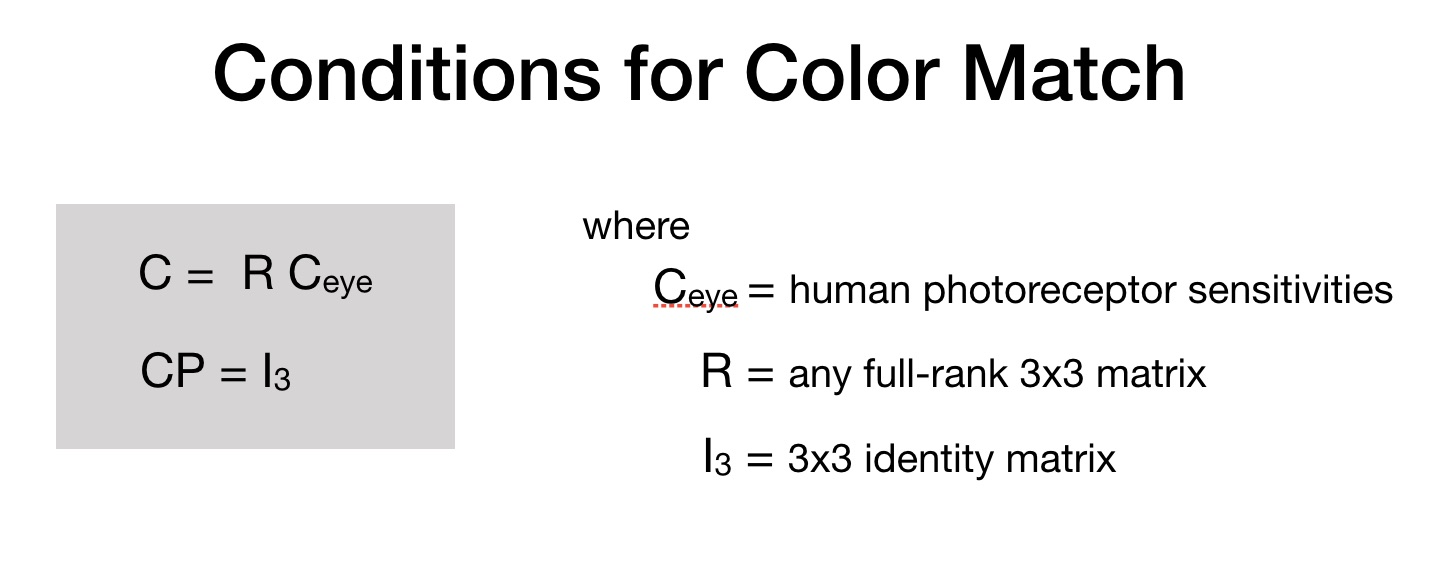
\epsfig{file=figures/color/conditions.jpg,width=4in}
%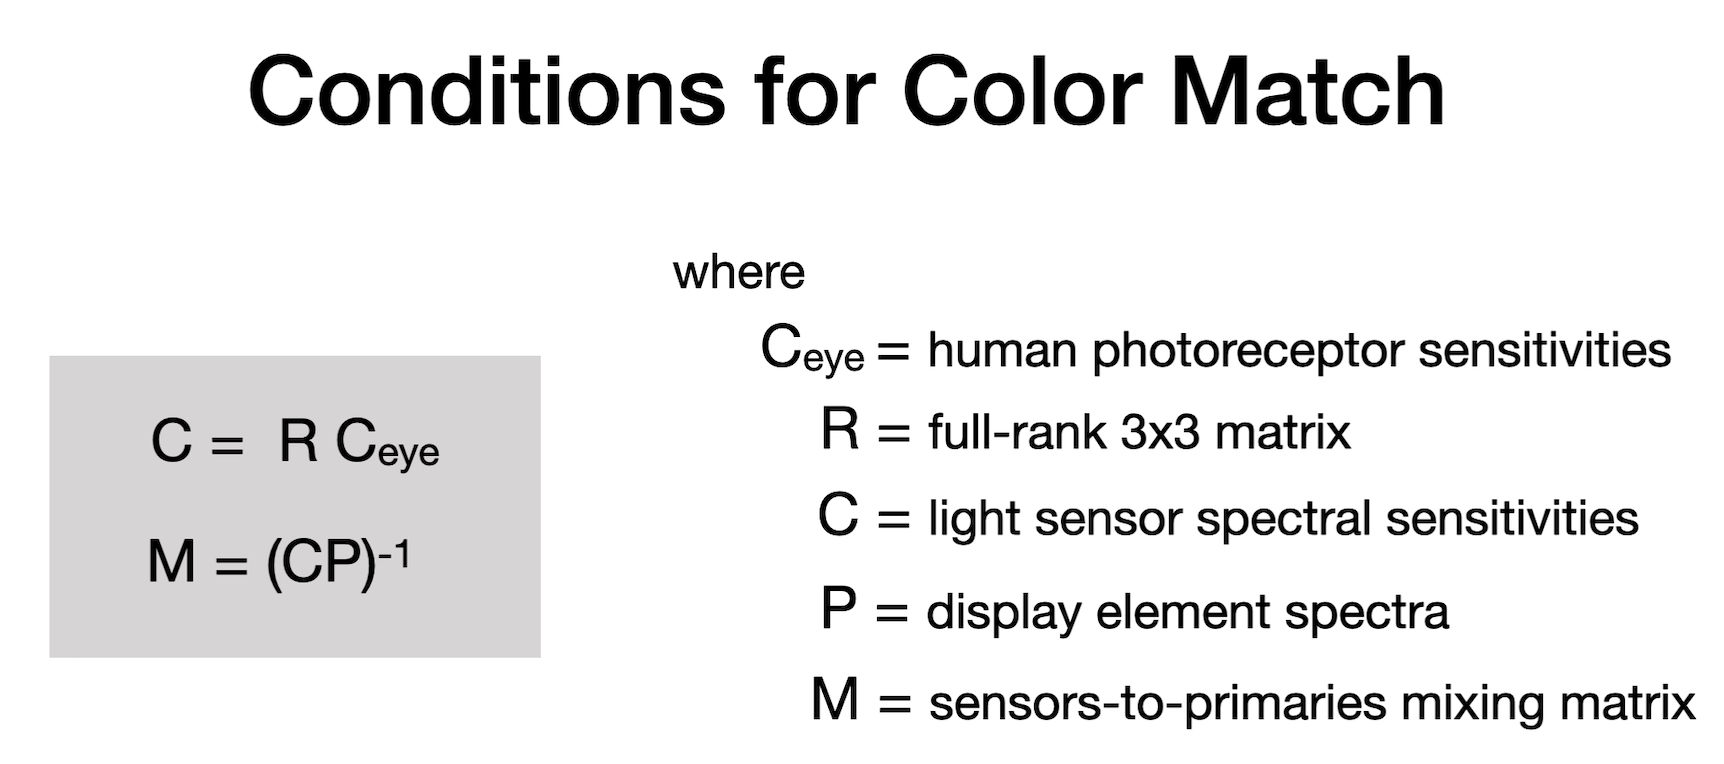
\epsfig{file=figures/color/conditionsForMatch.jpg,width=4in}
% }
% \caption{Conditions for a perceptual match for the system of Fig.~\ref{fig:colorsystem}.  First, $\mathbf{C}$ must be a linear combination of the spectral sensitivities of the photoreceptors in the eye, thus $\mathbf{C} = \mathbf{R} \mathbf{C}_{\mbox{eye}}$, for some full-rank, 3x3 matrix, $\mathbf{R}$.  Second, the light sensor spectra, in the rows of $\mathbf{C}$, and the display element spectra, in the columns of $\mathbf{P}$, must satisfy $\mathbf{C}\mathbf{P} = \mathbf{I}_{\mbox{3}}$.}
% \label{fig:conditions}
% \end{figure}

In this chapter, we assume that color appearance is determined by the light spectrum reaching the eye. In reality, numerous factors can influence color appearance, including the eye's state of brightness adaptation, ambient illumination, and surrounding colors. However, a color matching system that relies solely on the light spectrum will still perform well.

To measure the color associated with a light spectrum $\mathbf{t}$ we need to be able to predict the eye's responses to the spectrum.
From \eqn{\ref{eq:lmsct}}, the task of color measurement is to find the projection of a given light spectrum into the
special 3D subspace defined by the eye's cone spectral response curves.
Any basis for that 3D subspace will serve that task, so the three basis
functions do not need to be the color sensitivity curves of
\fig{\ref{fig:ramon}} themselves.  They can be any linear combination
of them, as well. 

We can define a {\bf color reproduction system}, \fig{\ref{fig:colorsystem}}, by first specifying its  three spectral sensitivity curves.  We put these into the $3 \times N$ matrix, $\mathbf{C}$, where $N$ is the number of spectral samples over the visible illumination range.  As discussed previously, the three curves, $\mathbf{C}$, should be a linear combination of the eye's spectral sensitivity curves, or
\begin{equation}
    \mathbf{C} = \mathbf{R} \, \mathbf{C}_{\mbox{eye}},
    \label{eq:match2}
\end{equation}
where $\mathbf{R}$ is any full-rank $3 \times 3$ matrix. We can translate between any two different color
spaces by  applying a general $3 \times 3$ matrix transformation
to change basis vectors.  Note, the basis vectors do not need to be
orthogonal, and  most color system basis vectors are not.


\begin{figure}[t]
\centerline{
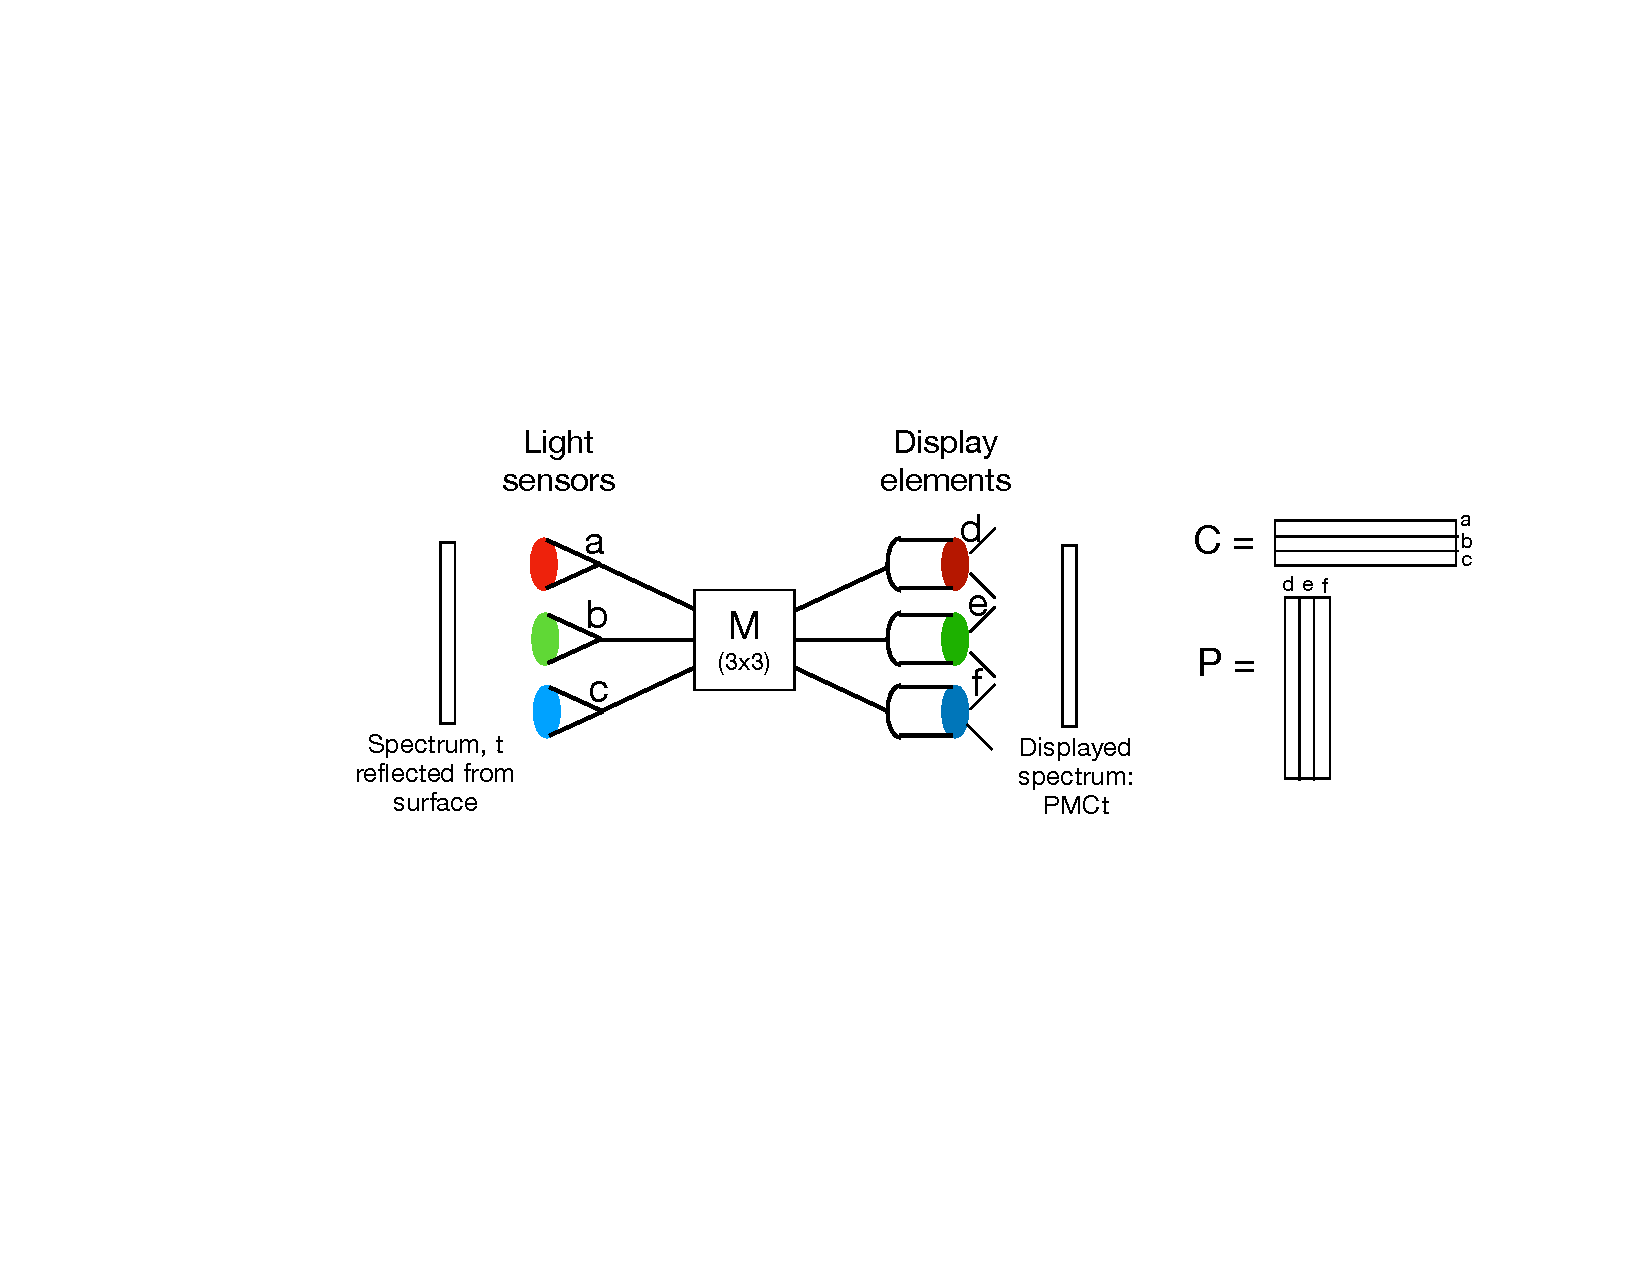
\includegraphics[width=1.0\linewidth]{figures/color/colorRepro2.pdf}
}
%\centerline{
%% 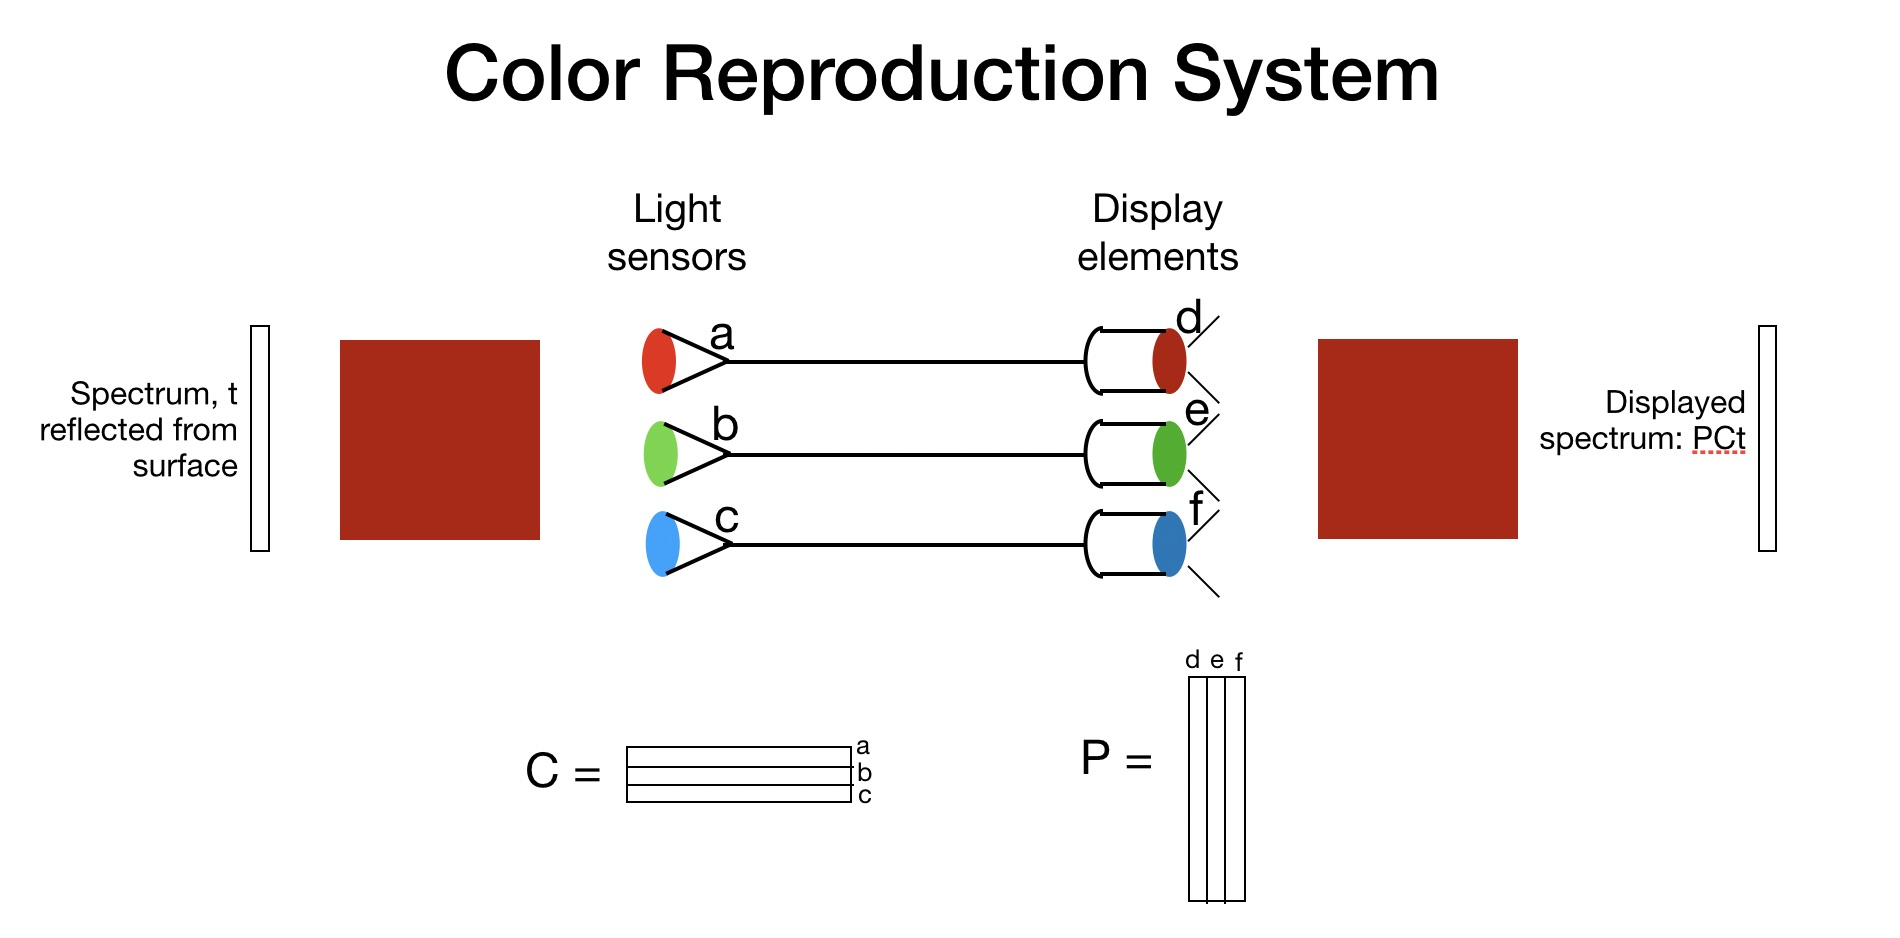
\epsfig{file=figures/color/colorsystem.jpg,width=5in}}
%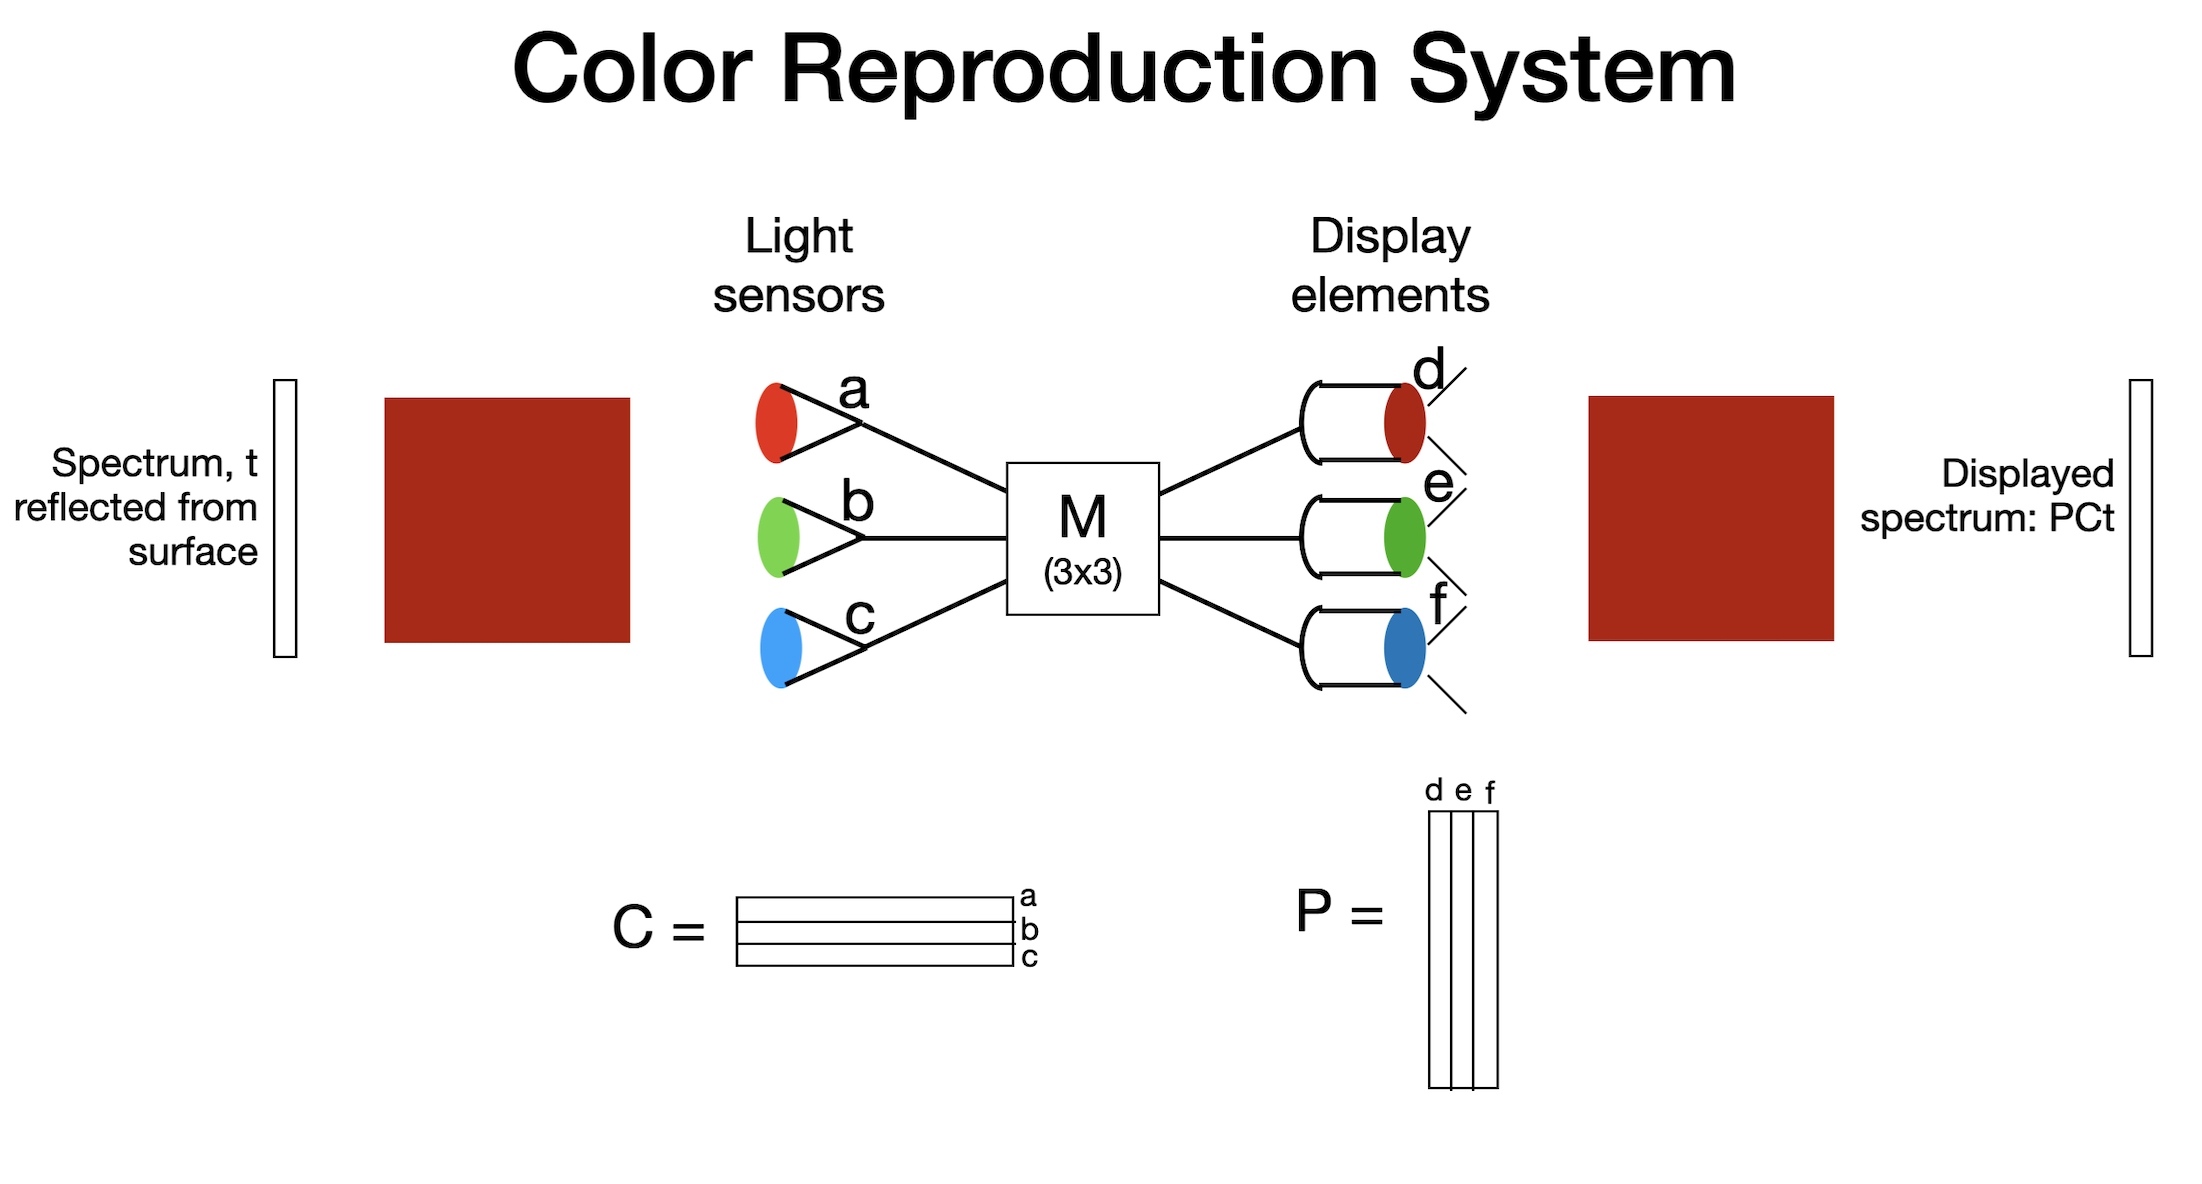
\epsfig{file=figures/color/colorRepro.jpg,width=5in}}
\caption{A color reproduction system.  Light sensors a, b, and c respond to the input light spectrum $\mathbf{t}$, giving sensor activations $\mathbf{C} \mathbf{t}$.  Combinations of those activations drive the display elements d, e, and f, producing the output spectrum $\mathbf{P}\mathbf{M} \mathbf{C} \mathbf{t}$. Conditions on $\mathbf{P}$, $\mathbf{M}$, and $\mathbf{C}$ can ensure that the input and output colors match for an observer.}
\label{fig:colorsystem}
\end{figure}


\subsection{Color Matching Functions and Primary Lights}

A  color reproduction system measures an input light and produces an output light that matches the color appearance of the input light.  A camera with a screen display is an example of a color reproduction system, as the colors of objects in the world are measured, then reproduced on the screen display of the camera.  
We can match the eye's response to a given light spectrum through the appropriate control of a sum of three lights, which we'll call the {\bf primary lights}\index{Color!Primary colors}. For the example of a display screen, the three color elements of each pixel are the primary lights.  

Because the eye's photosensors respond in linear proportion to the amount of the incoming light spectrum within its spectral sensitivity curve, the rules of linear algebra apply to color manipulation.  For a given set of three primary lights, the strengths of each primary light can be adjusted to obtain a visual match to a desired color.  There is one exception to this: because primary lights can only be combined in positive values, some input colors are outside the {\bf gamut}---the range of colors that can be produced---of a the positive combination of a given set of primary lights.

The color reproduction system is then defined by two sets of spectral curves and a $3 \times 3$ matrix, $\mathbf{M}$, see \fig{\ref{fig:colorsystem}}.  The first set are the spectral sensitivities as a function of wavelength for each of the three photosensors.  We write each of those spectral curves as a row vector of a matrix, $\mathbf{C}$.  The $3 \times 3$ matrix, $\mathbf{M}$, translates any color measurement to a set of amplitude controls for the primary lights, $\mathbf{P}$. The second set of spectral curves of a color reproduction system are the spectra of the three primary lights, which we write as column vectors of the matrix, $\mathbf{P}$.

For a given set of primary lights, $\mathbf{P}$, we seek to find a matrix of color sensitivity curves, $\mathbf{C}$, and $3 \times 3$ matrix, $\mathbf{M}$, which allow perfect reproduction of colors, as viewed by a human observer.  Here, we derive the conditions
%, given in \fig{\ref{eq:conditions}}, 
that $\mathbf{P}$,  $\mathbf{C}$, and $\mathbf{M}$ must satisfy to allow for perfect reproduction of colors.

Let the spectrum of the light reflecting from the surface to be matched in color be $\mathbf{t}$.  The eye's response to that light is modeled as the sum of a term-by-term multiplication of the spectral sensitivities of each photoreceptor, in the rows of $\mathbf{C}_{\mbox{eye}}$ times the spectrum of the light.  Thus, the responses of the eye to that spectrum will be the $3 \times 1$ column vector, $\mathbf{C}_{\mbox{eye}} \mathbf{t}$.  

We can write the response of the eye to the {\em output} of the color matching system as the following matrix products.  The light impinging on the sensors (a, b, c in \fig{\ref{fig:colorsystem}}) of the color matching system will give responses $\mathbf{C} \mathbf{t}$ and controls  $\mathbf{M} \mathbf{C} \mathbf{t}$ to the primary lights.  If this output modulates the corresponding primary lights (d, e, and f in \fig{\ref{fig:colorsystem}}), then the light displayed by the color matching system will be $\mathbf{P} \mathbf{M} \mathbf{C} \mathbf{t}$.  We want this spectrum to give the same responses in the eye as the original reflected color, thus we must have:
$\mathbf{C}_{eye} \mathbf{P} \mathbf{M} \mathbf{C} \mathbf{t} = \mathbf{C}_{eye} \mathbf{t} $.  Because that relation must hold for {\em any} input vector $\mathbf{t}$, we must have
\begin{equation}
\mathbf{C}_{eye} \mathbf{P} \mathbf{M} \mathbf{C}  = \mathbf{C}_{eye}   
\label{eq:match}
\end{equation}

What conditions on $\mathbf{P}$ and $\mathbf{C}$ are required for \eqn{\ref{eq:match}} to hold?  First, the subspace of the eye responses $\mathbf{C}_{eye}$ must be the same as that measured by the color sensing system, $\mathbf{C}$.  If that weren't the case, 
then perceptibly different spectra could map onto the same color sensing system measurements. So we must have $\mathbf{C} = \mathbf{R} \mathbf{C}_{eye}$, for some full-rank $3 \times 3$ matrix, $\mathbf{R}$ (with inverse $\mathbf{R}^{-1}$).  Substituting this twice into \eqn{\ref{eq:match}} gives
\begin{equation}
\mathbf{R}^{-1} \mathbf{C} \mathbf{P} \mathbf{M} \mathbf{R} \mathbf{C}_{eye} = \mathbf{C}_{eye}
\label{eq:match2}
\end{equation}
From \eqn{\ref{eq:match2}} it follows that  $\mathbf{C} \mathbf{P} \mathbf{M} = \mathbf{I}_3$, the $3 \times 3$ identity matrix.  These conditions on the spectral sensitivities, $\mathbf{C}$, the display spectra, $\mathbf{P}$ and the sensors-to-primaries mixing matrix, $\mathbf{M}$ for a color reproduction system are  summarized below:
\begin{eqnarray}
\mathbf{C} & = & \mathbf{R} \mathbf{C}_{\mbox{eye}} 
\label{eq:conditionsA} \\
\mathbf{M} & = & (\mathbf{C P})^{-1},
\label{eq:conditions}
\end{eqnarray}
where $\mathbf{C}_{\mbox{eye}}$ are the human photoreceptor sensitivities and $\mathbf{R}$ is a full-rank $3 \times 3$ matrix.  

%\marginnote{Conditions required for color matching in the color reproduction system of \fig{\ref{fig:colorsystem}}.}

\Fig{\ref{fig:exampleColor}} displays  the elements of two matrices $\mathbf{C}$ and $\mathbf{P}$ that define a valid color matching system.  For a color reproduction system to be physically realizable, the elements of the primary spectra, $\mathbf{P}$, must be non-negative.

% (In some color reproduction systems, there
% may be an additional 3x3 matrix Q multiplying the raw sensor spectral sensitivities to obtain the 
% color matching matrix C).



\begin{figure}[t]
\centerline{
\sublabelnp{(a)}{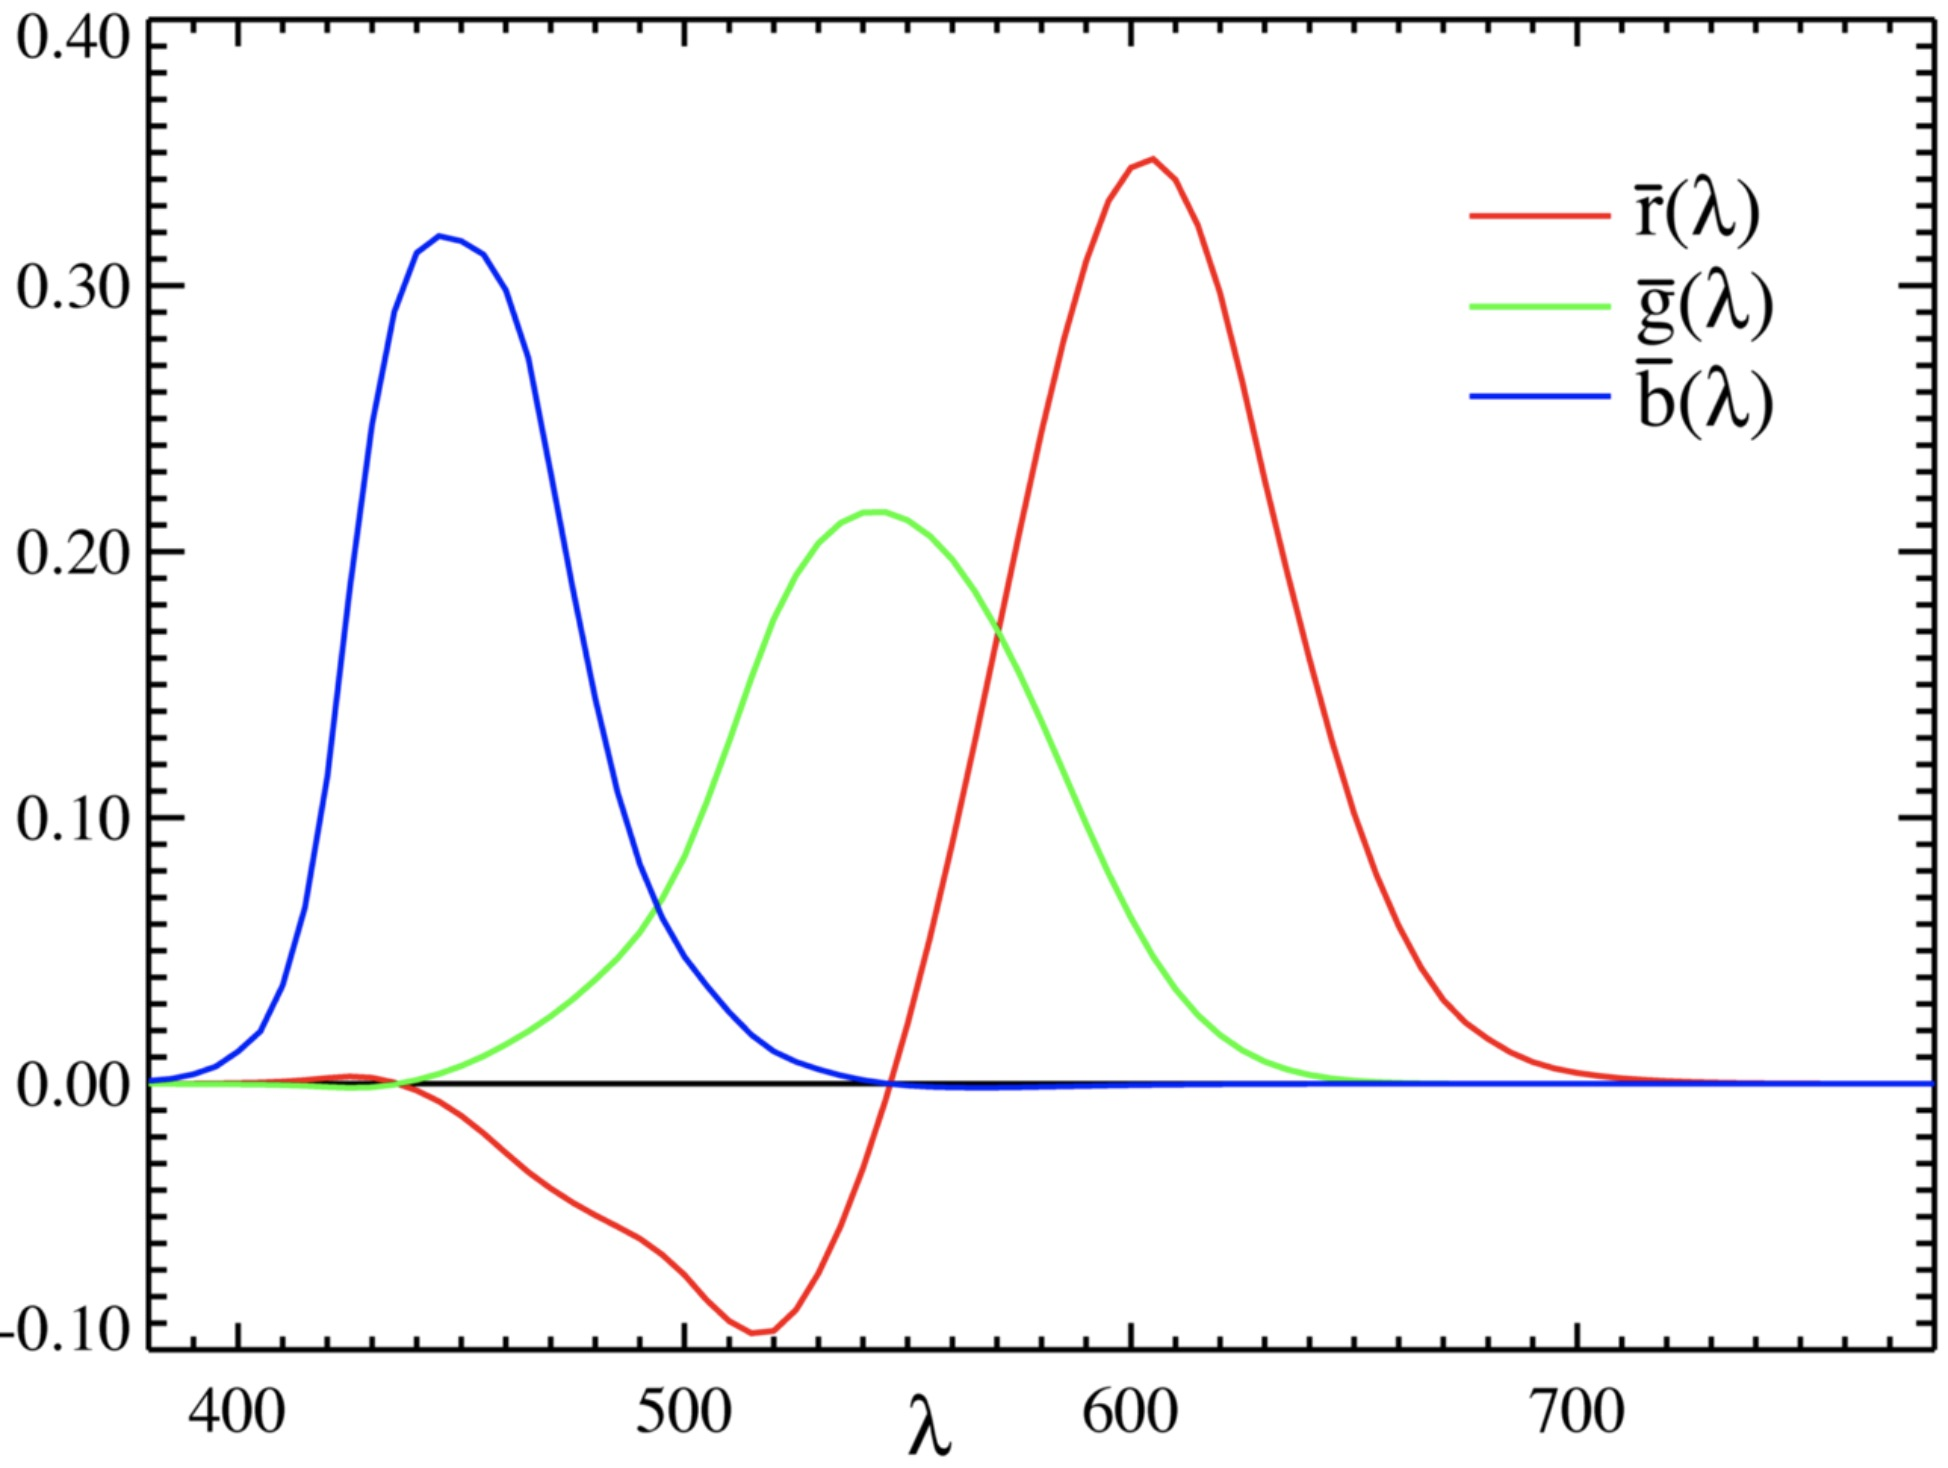
\epsfig{file=figures/color/ciergb.jpg,width=2.5in}}
\sublabelnp{(b)}{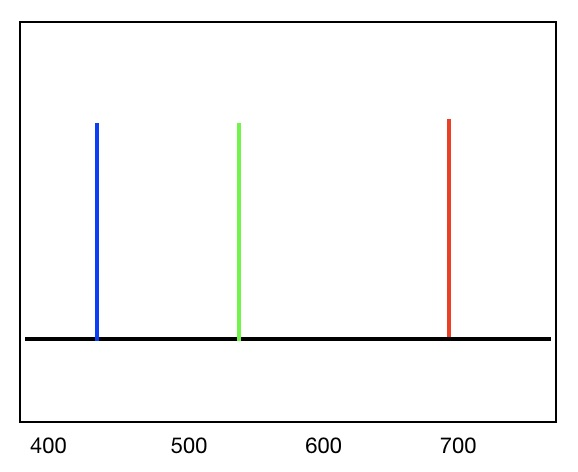
\epsfig{file=figures/color/primaryLights.jpg,width=2.5in}}}
\caption{The elements of the matrices $\mathbf{C}$ and $\mathbf{P}$ for an example color matching system.  (a) Spectral sensitivity curves, the rows of a color measurement matrix, $\mathbf{C}$. These should be linear combinations of the eye's photosensitivity curves, $\mathbf{C}_{\mbox{eye}}$.
(b) Corresponding primary lights, $\mathbf{P}$ \cite{Acdx2009},  satisfying $\mathbf{C} \mathbf{P}= \mathbf{I}_3$ ($\mathbf{M} = \mathbf{I}_3$  in equation [\ref{eq:conditions}]).}
\label{fig:exampleColor}
\end{figure}

Because many color sensitivity matrices $\mathbf{C}$ can satisfy \eqn{\ref{eq:conditionsA}} some standardized color sensitivity matrices have been adopted to allow common representations of colors. 


\subsection{CIE Color Space}

A color space is defined by the matrix, $\mathbf{C}$, with three rows
of color sensitivity functions.  These three sensitivity functions, $\mathbf{C}$, must be some linear combination of the sensitivity functions of the eye, $\mathbf{C}_{\mbox{eye}}$.
One color standard is the Commission Internationale de l'Eclairage (CIE) {\em XYZ} color space, $C_{\mbox{CIE}}$.  The CIE color matching functions, the rows of $\mathbf{C}_{\mbox{CIE}}$
were designed to be all-positive at every wavelength and are shown
in \fig{\ref{fig:ciecie}}.  


\begin{figure}[t]
\centerline{
{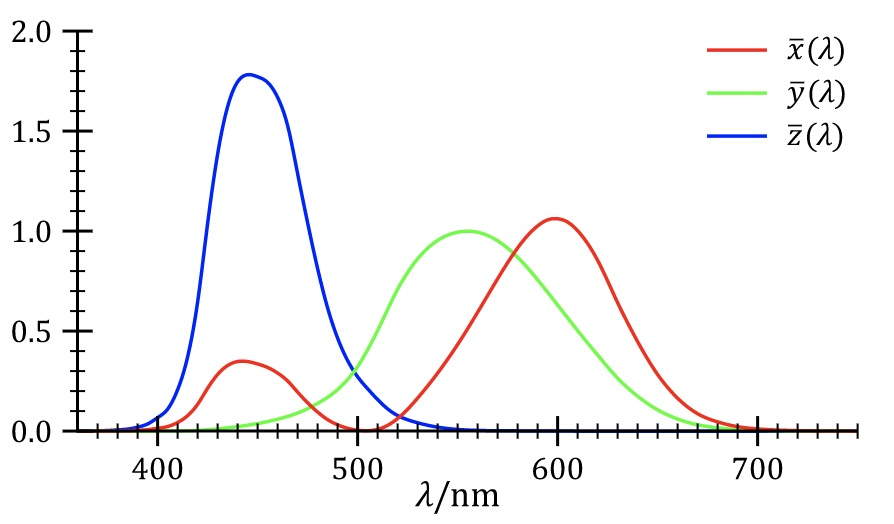
\epsfig{file=figures/color/ciecie.jpg,width=3in}}}
\caption{CIE color matching functions \cite{cie1931}.}
\label{fig:ciecie}
\end{figure}


An unfortunate property of the CIE color-matching functions is that no all-positive set of color primaries, $\mathbf{P}_{\mbox{CIE}}$ forms a color-matching system with those color-matching functions, $\mathbf{C}_{\mbox{CIE}}$.  But $\mathbf{C}_{\mbox{CIE}}$ is a valid matrix with which to measure colors, even though there is no physically realizable set of corresponding color primaries, $\mathbf{P}_{\mbox{CIE}}$.

To find the CIE color coordinates, one projects the input spectrum
onto the three color-matching functions, to find coordinates, called
tristimulus values, labeled $X$, $Y$, and $Z$.   Often, these values are
normalized to remove overall intensity variations, and one calculates {\bf CIE chromaticity coordinates}\index{Color!CIE chromaticity coordinates} $x = \frac{X}{X+Y+Z}$ and $y = \frac{Y}{X+Y+Z}$.



\begin{comment}
\begin{figure}[htpb!]
\centerline{
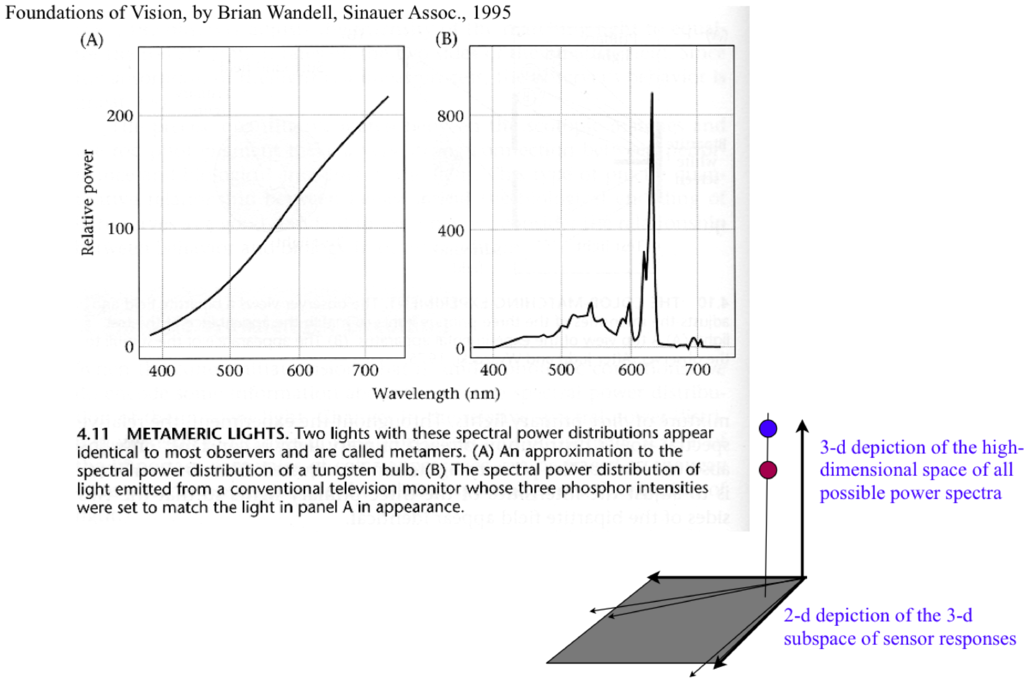
\epsfig{file=figures/color/metamerism.eps,width=6in}}
\caption{The two spectra in the figure above, from \cite{Wandell95},
  are colors that match perceptually:  daylight, and the spectrum a
  monitor adjusted to match daylight.    The figure at right shows a
  graphical rendition of the projection from the high-dimensional
  space of power spectra onto a lower-dimensional subspace,
  representing the 3D space of human color perception.  The red and
  blue dots in the higher-dimensional space are ``metameric'' in that
  they project to the same location in the lower-dimensional subspace.}
\label{fig:metamerism}
\end{figure}
\end{comment}

\begin{comment}
Let us summarize our discussion of color so far.  Under certain
viewing conditions, the perceived color depends just on the spectral
composition of light arriving at the eye (we move to more general
viewing conditions next).  Under such conditions, there is a simple
way to describe the perceived color:  project its power spectrum onto
a set of 3 vectors called color matching functions.  These projections
are the color coordinates.  
We standardize on particular sets of color coordinates.  One such set
is the CIE XYZ system.  
\end{comment}

\begin{comment}
How do you translate from one set of color coordinates
to another, say, for notation, from the color coordinates in a unprimed system to those
in a primed system?   Place the spectra of a set of primary lights
into the columns of a matrix ${\bf P}$.  If we take the color
coordinates, $\mathbf{x}$, as a 3x1 column vector and multiply them by the matrix
${\bf P}$, we get a spectrum which is metameric with the input
spectrum whose color coordinates were $\mathbf{x}$.  So to convert
$\mathbf{x}$ to its representation in a primed coordinate system, we just
have to multiply this metameric spectrum by  the color matching
functions for the primed color system:
\begin{equation}
\mathbf{x}' = {\bf C}'{\bf P} \mathbf{x}
\end{equation}
The color translation matrix ${\bf C}'{\bf P}$ is a 3x3 matrix.
\end{comment}



%% When did people learn that we have three color receptors, and how did
%% they find out?  ((   read about it.        ))



\begin{comment}

\subsection{Color mixing}

In art or photography, we often talk of ...      (relate to color primaries).


\begin{figure}[htpb!]
\centerline{

\epsfig{file=figures/color/yellowgreen.eps,width=1.5in}}
\caption{The cyan of Windex and the yellow of Joy combine to give a
 green color.}
\label{fig:colormixing}
\end{figure}

Colors and color mixing are a delightful aspect of our visual experience.
Fig.~\ref{fig:colormixing} shows an everyday example of color mixing:
yellow and cyan colors combining to give a green. 

Physically, color mixing involes combining the spectra of the two
colors to be mixed to create the power spectrum of the mixed color.
Various processes cause colors to mix, but the results
can be divided into two broad classes of mixing, called additive and
subtractive.  Under additive color mixing, the
power spectra add together to form the spectrum of the resulting
color.  This model of mixing covers the case of many small color 
elements for which the appearance is fused, such as tiny elements of a
display, or the case of several light projectors pointing at the same screen.
CRT color televisions, DLP projectors, and
colors viewed very closely in space or time all exhibit additive color
mixing.  The spectrum of the mixed color is a weighted sum of the
spectra of the individual components.  In the additive
color mixing model, red and green combine to give yellow, as can be
seen from the cartoon models of Figs.~\ref{fig:names} and
\ref{fig:colormixing}. 

A second way colors combine is called subtractive color mixing, but
might better be called multipliciative color mixing.  Under this
mixing model, the spectrum of the combined color is proportional to
the {\em product} of the mixed components.  This color mixing occurs
when light of one color reflects diffusely off a surface of another
color, or passes through a sequence of attenuating spectral filters,
such as with photographic film, paint, optical filters, and crayons.
Under the subtractive color mixing model, cyan and yellow combine to
give green, since the cyan filter attenuates the red components of
white light, and yellow filter would remove the remaining blue
components, leaving only the green spectral region of the original
white light.  Under subtractive color mixing,  red and green combine to give black.

Figure~\ref{fig:mixing} shows examples of color mixing.

\begin{figure}[htpb!]
\centerline{
\sublabel{a}{\epsfig{file=figures/color/additiveMixing.eps,width=3in}}
\sublabel{b}{\epsfig{file=figures/color/subtractiveMixing.eps,width=3in}}}
\caption{Examples of color mixing, in the world of cartoon color spectra.  (a) Additive, (b) subtractive.  The
 spectra and the resulting colors.}
\label{fig:mixing}
\end{figure}


Because the spectrum depends on surfaces, it is very useful to measure
the spectrum of reflected light, and we discuss how the eye does that
in the following section.

\end{comment}



\section{Spatial Resolution and Color}

Color interacts with our perception of spatial resolution.  For some directions in color space, the eye is very sensitive to fine spatial modulations, while for other color space directions, the eye is relatively insensitive.  Some color coordinate systems take advantage of this disparity to enable efficient representation of images by sampling image data sparsely along color axes where human perception is insensitive to blurring.

In a red-green-blue (RGB) representation, the eye is sensitive to high spatial frequency changes in both red and green, as shown in figures \ref{fig:girls1} and \ref{fig:girls2}.  A rotation of the color coordinates of the image, followed by a nonlinear stretching, can put the image into a color space called L, a, b\index{Color!Lab space}.  In that space, the eye is very sensitive to any blurring of the L color component, called luminance, but is relatively insensitive to blurring of the a or b components, as demonstrated in \fig{\ref{fig:girls3}} and \ref{fig:girls4}.  This effect is commonly exploited in image compression, allowing some image components to be sampled more coarsely than others.


\begin{figure}
\centerline{
\includegraphics[width=1.0\linewidth]{figures/color/nonblur_girls.eps}
}
%\centerline{
%\sublabelnp{(a) Original}{\epsfig{file=figures/color/nonblur.eps,width=2.3in}}
%\sublabelnp{(b) R, G, B components}{\epsfig{file=figures/color/rgbgirls.eps,width=2.3in}}
%\sublabelnp{(c) blurred R, G, B components}{\epsfig{file=figures/color/blurrgbgirls.eps,width=2.0in}}}
\caption{(a) Original image.  (b) RGB components.  (c) RGB components,
  each blurred.  These sharp and blurred components are used  in the color images of \fig{\ref{fig:girls2}}.
}
\label{fig:girls1}
\end{figure}



\begin{figure}
\centerline{
\includegraphics[width=1.0\linewidth]{figures/color/blur_rgb_girls.eps}
}
%\centerline{
%\sublabelnp{(a) R component blurred}{\epsfig{file=figures/color/blurrgirls.eps,width=2.3in}}
%\sublabelnp{(b) G component blurred}{\epsfig{file=figures/color/blurggirls.eps,width=2.3in}}
%\sublabelnp{(c) B component blurred}{\epsfig{file=figures/color/blurbgirls.eps,width=2.3in}}}
\caption{Color images composed of sharp and blurred components from figures \ref{fig:girls1}(b) and \ref{fig:girls1}(c).  (a) R component blurred, G and B components sharp.  (b)  G component blurred, R and B components sharp. (c) B component blurred, R and G components sharp. Blurring either the R or G components of the image leads to a blurry-looking full-color image.
}
\label{fig:girls2}
\end{figure}

\begin{comment}
\begin{figure}[htpb!]
\centerline{
\epsfig{file=figures/color/rgbyiq.eps,width=3in}}
\caption{Human spatial frequency sensitivity in R, G, B and L, a, b
  color representations
}
\label{fig:sensitivity}
\end{figure}
\end{comment}




\begin{figure}
\centerline{
\includegraphics[width=1.0\linewidth]{figures/color/nonblur_lab_girls.eps}
}
%\centerline{
%\sublabelnp{(a) Original}{\epsfig{file=figures/color/nonblur.eps,width=2.3in}}
%\sublabelnp{(b) L, a, b components}{\epsfig{file=figures/color/labgirls.eps,width=2.3in}}
%\sublabelnp{(c) blurred L, a, b components}{\epsfig{file=figures/color/blurlabgirls.eps,width=2.3in}}}
\caption{(a) Original image.  (b) Lab components.  (c) Lab components,
  each blurred.   These sharp and blurred components are used  in the color images of \fig{\ref{fig:girls4}}.
}
\label{fig:girls3}
\end{figure}



\begin{figure}
\centerline{
\includegraphics[width=1.0\linewidth]{figures/color/blur_lab_girls.eps}
}
%\centerline{
%\sublabelnp{(a) L component blurred}{\epsfig{file=figures/color/blurlgirls.eps,width=2.3in}}
%\sublabelnp{(b) a component blurred}{\epsfig{file=figures/color/bluragirls.eps,width=2.3in}}
%\sublabelnp{(c) b component blurred}{\epsfig{file=figures/color/blurbbgirls.eps,width=2.3in}}}
\caption{Color images composed of sharp and blurred components from figures \ref{fig:girls3}(b) and \ref{fig:girls3}(c).  (a) L component blurred, a and b components sharp.  (b)  a component blurred, L and b components sharp. 
(c) b component blurred, L and a components sharp. Blurring only either of the a or b components of the image yields a full-color image that appears sharp, provided the luminance component of the image is sharp.}
\label{fig:girls4}
\end{figure}





\begin{comment}

\subsection{Low-dimensional models for spectra}

Before we turn to color perception, let's introduce a mathematical
model for light spectra that makes them much easier to work with.  In
general, when modeling the world, we want to keep everything as simple
as possible, and that usually means working with as few degrees of freedom as
possible.   Color spectra seem like relatively high-dimensional
objects, since we can pick any combination of numbers, from 400 to 700
nm, as we'd like.  Even sampling at every 10 nm of wavelength, that
gives us 31 numbers for each spectrum.

It turns out that for many real-world spectra, those 31 numbers are not
independent and in practise spectra have far fewer degrees of freedom.
It is common to use low-dimensional linear models to approximate
real-world reflectance and illumination spectra.   Any given spectrum, say
$S(\lambda)$, is approximated as some linear combination of ``basis
spectra'', $u(\lambda)$.  For example, a 3-dimensional linear model of $S(\lambda)$
would be
\begin{equation} 
\left( 
\begin{array}{c}
\vdots \\
S(\lambda) \\
\vdots
\end{array}
\right) 
\approx
\left( 
\begin{array}{ccc}
\vdots  & \vdots & \vdots \\
u_1 (\lambda)  & u_2 (\lambda)  & u_3 (\lambda)  \\
\vdots & \vdots & \vdots 
\end{array}
\right) 
\left( 
\begin{array}{c}
\omega_1 \\
\omega_2 \\
\omega_3
\end{array}
\right) 
\label{eq:lowd}
\end{equation} 

The basis spectra can be found from a collection of training spectra.
If we write the training spectra as columns of a matrix, $D$, then
performing a singular value decomposition on $D$ yields
\begin{equation}
D = U * \Lambda * V'
\end{equation}
where $U$ is a set of orthonormal spectral basis vectors, $\Lambda$ is a
diagonal matrix of singular values, and $V'$ is a set of
coefficients.  The first $n$ columns of $U$ are the $n$ basis spectra that
can best approximate the spectra in the training set, in a least
squares sense.

Here's a demonstration, with a particular collection of
surface reflectance spectra, $u_i(\lambda)$ that this works quite well.  The ``Macbeth
Color Checker'', a tool of color scientists and engineers,
 is a standard set of 24 color tiles, made the same way year after
 year.  (So iconic that this woman, a dedicated color scientist, I
 presume, has tatooed a Macbeth color checker on her arm!  Alas, I'm
 sure the tatoo colors are only an approximation to the real Macbeth colors).

The reflectance spectra of each Macbeth color chip has been measured.
All those spectra are pretty well approximated by a 3-dimensional
linear model, as you can see from these plots.


\begin{figure}[htpb!]
\centerline{
\epsfig{file=figures/color/macbeth.eps,width=3in}
\epsfig{file=figures/color/macbethTatoo.eps,width=2.5in}}
\centerline{
\epsfig{file=figures/color/macbethBases.eps,width=4in}
\epsfig{file=figures/color/macbethApprox.eps,width=4in}}
\caption{Macbeth color checker. iconic status.  spectra.  bottom two
  figures from Foundations of Vision, by Brian Wandell, Sinauer Assoc., 1995
}
\label{fig:Macbeth}
\end{figure}



\section{Color Constancy}
\label{sect:colorconstancy}

Color perception depends strongly on the power spectrum of the light
arriving at the eye, but it does not depend only on that.  
Now we address the
assumption that a given spectral power distribution always leads to
the same color percept.

In the color constancy demo of Fig.~\ref{fig:cc}, we'll show an example where the identical
spectral distribution arriving at your eye leads to a very different
color percept.  What's going on?   The visual system needs to perceive
the color of surfaces, but the data it gets is the
wavelength-by-wavelength product of the
surface color and the illuminant color.  So our visual system needs to
``discount the illuminant'' and present a percept of the underlying colors
of the surfaces being viewed, rather than simply summarizing the
spectrum arriving at the eye.


\begin{figure}[htpb!]
\vspace{2in}
%% \centerline{
%% \sublabelnp{(c) b component blurred}{\epsfig{file=figures/color/blurbbgirls.eps,width=2.5in}}}
\caption{color constancy demo
}
\label {fig:cc}
\end{figure}


The ability to perceive or estimate the surface colors of the objects
being viewed, and to not be fooled by the illumination color, is called
``color constancy''--you perceive a constant color, regardless of the
illumination.  People have some degree of color constancy, although
not perfect color constancy.   

For the case where there is just one illumination color in the image,
if we know either the illuminant or all the surface colors, we can
estimate the other from the data.  So, from a computational point of
view, you can also think of the color constancy task as that of
estimating the illuminant spectrum from an image.

\subsubsection{The rendering equation}

Let's examine the computation required to achieve color constancy.
Here's the rendering equation, showing, in our model, how the L, M,
and S cone responses for the $j$th patch are generated:
\begin{equation}
\left( 
\begin{array}{c}
L_j \\
M_j \\
S_j
\end{array}
\right)
=
{\bf E}^T 
( {\bf A} \mathbf{x}^s_j
.*
 {\bf B} \mathbf{x}^i )
\label{eq:rendering}
\end{equation}
Figure~\ref{fig:graph} shows a graphical diagram showing the vector and
matrix sizes that I hope makes things a little clearer.  We have some
unknown illuminant, described by, say, a 3-dimensional vector of
coefficients for the illumination spectrum basis functions.  For this
$j$th color patch, we have a set of surface reflectance spectrum basis
coefficients, let's say also 3-dimensional.  The term-by-term product
of the resulting spectra (the quantity in parenthesis in the top
equation) is our model of the spectrum of the light reaching our eye.
That spectrum then gets projected onto spectral responsivity curves of
each of the three cone classes in the eye, resulting in the L, M, and
S response for this $j$th color patch.
(An equation for the RGB pixel color values would be the same, with just a different
matrix ${\bf E}$).   If we make $N$ distinct color
measurements of the image, then we'll have $N$ different versions of
this equation, with a different vector $\mathbf{x}^s_j$ and different
observations 
$\left( 
\begin{array}{c}
L_j \\
M_j \\
S_j
\end{array}
\right) 
$ for each equation.


\begin{figure}[htpb!]
\centerline{
\epsfig{file=figures/color/graph.eps,width=5in}}
\caption{Graphical depiction of Eq.~\ref{eq:rendering}.
}
\label {fig:graph}
\end{figure}



Like various other problems in vision, this is a bilinear problem.  If
we knew one of the two sets of variables, we could find the other
trivially by solving a linear equation (using either a least squares
or an exact solution).  
It's a very natural generalization of the $a b = 1$ problem.

Let's notice the degrees of freedom.  We get 3 numbers for every new
color patch we look at, but we also add 3 unknowns we have to estimate
(the spectrum coefficients $\mathbf{x}^s_j$), as well as the additional
three unknowns for the whole image, the illumination spectrum
coefficients $\mathbf{x}^i$.  If only surface color spectra had only two
degrees of freedom, we'd catch up and potentially have an
over-determined problem if we just looked at enough colors in the
scene.  Unfortunately, 2-dimensional surface reflectance models just
don't work well in practice.


\subsection{Some color constancy algorithms}
So how will we solve this?  Let's look at two well-known simple algorithms,
and then we'll look at a Bayesian approach.

{\bf Bright equals white}
If we knew the true color of even a single color patch, we'd have the
information we needed to estimate the 3-d illumination spectrum.  One
simple algorithm for estimating or balancing the illuminant is to
assume that the color of the brightest patch of an image is white.  (If you're working
with a photograph, you'll always have to worry about clipped intensity
values, in addition to all the non-linearities of the camera's
processing chain).   If that is the $k$th patch, and $\mathbf{x}^W$ are
the known spectral basis coefficients for white, 
then we have
\begin{equation} 
\mathbf{y}_k =
\left( 
\begin{array}{c}
L_k \\
M_k \\
S_k
\end{array}
\right) 
=
{\bf E}^T 
({\bf A} \mathbf{x}^W 
\hspace{1mm} .* \hspace{1mm}
{\bf B}\mathbf{x}^i)
\end{equation} 
which we can solve for the unknown illuminant, $\mathbf{x}^i$.


How well does it work?  It works sometimes, but not always.  On the
left is a picture for which the bright equals white algorithm would
probably work (although I haven't checked it.  On the right is one
where I don't think it would work.

The bright equals white algorithm
estimates the illuminant based on the color of a single patch, and we
might expect to get a more robust illuminant estimate if we use many
color patches in the estimate.  A second heuristic that's often used
is called the {\bf grey world assumption}:  the average value of every
color in the image is assumed to be grey.


\begin{figure}[htpb!]
\centerline{
\epsfig{file=figures/color/nongrey.eps,width=2.5in}}
\caption{An image that violates the grey world assumption.}
\label {fig:nongrey}
\end{figure}




Taking the sum over all samples $j$ on both sides of
the rendering equation, and letting $\mathbf{x}^{G}$ be the spectral
basis coefficients for grey, gives
\begin{eqnarray} 
\frac{1}{N}
\sum_j 
\left( 
\begin{array}{c}
L_j \\
M_j \\
S_j
\end{array}
\right) 
& = & 
{\bf E}^T 
({\bf A} 
\frac{1}{N}
\sum_j \mathbf{x}^s_j 
\hspace{1mm} .* \hspace{1mm}
{\bf B}\mathbf{x}^i) \\
& = & 
{\bf E}^T 
({\bf A} \mathbf{x}^{G} 
\hspace{1mm} .* \hspace{1mm}
{\bf B}\mathbf{x}^i) \\
\label{eq:renderavg}
\end{eqnarray} 
Then, again, we just have a linear equation to solve for $\mathbf{x}^i$.

This assumption can work quite well, although, of course, we can find
images for which it would completely mess up, such as this forest
scene here.


Using just part of the data (the brightest color, or the average
color) gives sub-optimal results.  Why not use all the data, make a
richer set of assumptions about the illuminants and surfaces in the
world, and treat this as a {\bf Bayesian estimation problem}?  That's what
we'll do now, and what you'll continue in your homework assignment.


To remind you, in a Bayesian approach, we seek to find the posterior
probability of the state we want to estimate, given the observations
we see.  We use Bayes rule to write that probability as a (normalized)
product of two terms we
know how to deal with:  the likelihood term and the prior term.
Letting $\mathbf{x}$ be the quantities to estimate, and $\mathbf{y}$ be the
observations, we have
\begin{equation}
P(\mathbf{x} | \mathbf{y}) = k P(\mathbf{y} | \mathbf{x} ) P(\mathbf{x}) 
\label{eq:bayes}
\end{equation}
where $k$ is a normalization factor that forces that the integral of
$P(\mathbf{x}|\mathbf{y})$ over all $\mathbf{x}$ is one.

The likelihood term tells us, given the model, how probable the
observations are.  If we assume additive, mean zero Gaussian noise, the
probability that the $j$th color observation differs from the rendered parameters
follows a mean zero Gaussian distribution.  Remembering that the observations $\mathbf{y}_j$
are the the L, M, and S cone responses, 
\begin{equation}
\mathbf{y}_j
=
\left( 
\begin{array}{c}
L_j \\
M_j \\
S_j
\end{array}
\right)
\end{equation}

we have
\begin{equation} 
P(\mathbf{y}_j | \mathbf{x}^i, \mathbf{x}^s_j) = \frac{1}{\sqrt{2 \pi \sigma^2}} \exp{\frac{-|
\mathbf{y}_j
-
  \mathbf{f}(\mathbf{x}^i, \mathbf{x}^s_j)|^2}{2 \sigma^2}},
\label{eq:likelihood}
\end{equation} 

For an entire collection of $N$ surfaces, we have
\begin{equation}
P(\mathbf{x} | \mathbf{y}) =
P(\mathbf{x}^i)
\prod_j
P(
\mathbf{y}_j
| \mathbf{x}^i, \mathbf{x}^s_j) 
P(\mathbf{x}^s_j) 
\end{equation}




{\bf reminder:}
Here's what's inside the rendering function, 
$\mathbf{f}(\mathbf{x}^i, \mathbf{x}^s_j)$.  We  assume diffuse reflection from each
colored surface.  Given basis function coefficients for the illuminant, 
$\mathbf{x}^i$, and a matrix ${\bf B}$ with the illumination basis
functions as its columns, then the spectral illumination as a function
of wavelength is the column vector ${\bf B}\mathbf{x}^i$.  
We also need to compute
$j$th surface's
diffuse reflectance spectral attenuation function, the product of its basis coefficients
times the surface spectral basis functions:
${\bf A} \mathbf{x}^s_j$
In our diffuse
rendering model, the reflected power is the term-by-term
product (we borrow Matlab notation for that, .*) of those two.  The
observation of the $j$th color is the projection of that spectral
power onto the eye's photoreceptor response curves.  If those
photoreceptor responses are in the columns of the matrix, ${\bf E}$,
then the forward model for the three photoreceptor responses at the
$j$th color is:
\begin{equation} 
\mathbf{f}(\mathbf{x}^i, \mathbf{x}^s_j)
=
{\bf E}^T 
({\bf A} \mathbf{x}^s_j 
\hspace{1mm} .* \hspace{1mm}
{\bf B}\mathbf{x}^i).
\label{eq:render}
\end{equation} 


\subsubsection{Eq.~(\ref{eq:render}), in component form}
We can find the linear solution of
Eq.~(\ref{eq:render}), for a given illuminant vector, $\mathbf{x}^i$, and
assuming no noise in the observations.
Let's write everything out in component form, in order to do the
calculation carefully.  Let's assume we're only fitting the $x^s_{kj}$
to the $j$th color patch observation, and therefore omit all
subscripts $j$, for simplicity.  So $x^s_{k}$ will mean the $k$th
reflectance basis component (of the $j$th patch).  $w$ indexes
wavelength values.
\begin{eqnarray} 
y_n & = &  
\sum_w E_{nw}  \sum_k   A_{wk} x^s_{k}
\sum_m
B_{wm} x^i_{m} \\
& = & 
\sum_k   
x^s_{k}
\sum_w E_{nw}  
A_{wk} 
\sum_m
B_{wm} x^i_{m} \\
\end{eqnarray} 
If we define the n, k components of a matrix D to be
\begin{equation}
D_{nk} = \sum_w E_{nw}  
A_{wk} 
\sum_m
B_{wm} x^i_{m} ,
\end{equation}
then we have
\begin{equation}
\mathbf{y}
=
{\bf D}  \mathbf{x}^s
\end{equation}
If ${\bf D} $ is invertible, then we have
\begin{equation}
\mathbf{x}^s
=
{\bf D^{-1}} \mathbf{y}
\end{equation}


\begin{figure}[htpb!]
\centerline{
\epsfig{file=figures/color/abproblem.eps,width=2.2in}}
\caption{y = ab problem}
\label{fig:yab}
\end{figure}




I want to remind us about the similarities between the 1 = ab problem,
and our color constancy problem.  While we can't draw out the
high-dimensional likelihood function for the color constancy problem,
conceptually it's very similar to that of this 1=ab problem (and
various other vision problems share these same characteristics).  Many
different settings of the parameters can explain our data, giving what
we call a ``likelihood ridge''.  For the 1=ab problem, that gives a
1-d ridge of parameter settings that explain the same data.  For the
color constancy problem, with 3-d data, surface parameterizations and
illuminant parameterization, the likelihood ridge is 3-dimensional.

How do we pick from the many feasible solutions on the ridge, all
with the same likelihood value?  The priors will let us distinguish
different values on the likelihood ridge.  

In the problem set, you'll fit Gaussians to model the observed prior
distribution of surface and illuminant basis function coefficients.

Another difference for different positions along the likelihood ridge
is the ``width'' of the ridge.  At some positions, only a very precise
specification of all the parameter values will explain the
observations.  At other positions, we have more slop in the
parameters, and many different nearby parameter settings also explain
the data.  In a Bayesian framework, this is most naturally quantified
with the {\bf loss function}, which specifies the penalty for guessing
wrong.  Let $\hat{\mathbf{x}}$ be your estimate of the parameters,
$\mathbf{x}$.  Then $L(\hat{\mathbf{x}}, \mathbf{x})$ is the loss incurred by
guessing $\hat{\mathbf{x}}$ when the true value was $\mathbf{x}$.  With the
posterior probability, we can calculate the expected loss, $\bar{L}(\hat{\mathbf{x}}, \mathbf{x})$
\begin{equation}
\bar{L}(\hat{\mathbf{x}}, \mathbf{x})
=
\int_{\mathbf{x} }L(\hat{\mathbf{x}}, \mathbf{x}) P(\mathbf{x} | \mathbf{y})
\end{equation}
We often use a loss function which is only a function of 
$\hat{\mathbf{x}} -\mathbf{x}$.


Bayes rule lets us find a posterior probability for $\mathbf{x}$, given
the observations $\mathbf{y}$.  The final stage of Bayesian estimation is
to go from that function, $P(\mathbf{x} |\mathbf{y})$, to a single best
guess value, $\hat{\mathbf{x}}$, a point estimate.

The two most commonly used point estimates are called the MAP and MMSE
estimates, and in your homework for this material, you'll use either
one of those for this color constancy problem.

The MAP estimate stands for ``maximum a posteriori'', Latin for
``just take the max of the posterior distribution''.  While quite a
natural thing to do, it can suffer from various problems, since it
only depends on the single maximum valued point of the posterior
probability.  The loss function implied by the MAP estimate assigns a
constant penalty for all guesses, except for a precisely correct
guess, which receives high reward.  This penalty structure doesn't
make sense for perceptual tasks, for which nearly the right answer is
often just as good as precisely the right answer.

Another very common estimate is MMSE, ``minimum mean squared error''.
This is the mean of the posterior probability, which, as the name
implies results in an estimate which minimizes the expected squared
error in the estimated parameter.  The homework assignment, excerpted
on these slides, gives details of how to find each of those estimates
for this problem.  Again, for perceptual problems, this loss function
often doesn't make sense, although in practice an MMSE estimate is
often very good.  (Although for the 1 = ab problem, limited to $0 < a, b< 4$,
the MMSE estimate is relatively far away from any feasible solution to
the problem).

\end{comment}


\begin{comment}
To control for those variables, care must be taken to
view the color comparisons under repeatable, controlled surrounding
colors.  We shine a controllable combination of the primary lights on
one half of a bipartite white screen, and the test light on the other
half.  A grey surround field is placed around the viewing aperture,
giving a view to the subject that looks something like that of
Fig.~\ref{fig:matching}~(a), right hand side (from \cite{Wandell95}).
We assign a triplet of numbers to the color appearance of a surface:
the amount of each of the three primary colors that is required to
match a given test color.


%% \billf{Now we just need to standardize on a set of primaries.}


\subsection{Box:  Color matching experiments}

\begin{figure}[htpb!]
\centerline{
\sublabel{a}{\epsfig{file=figures/color/colorMatchA.eps,width=5in}}}
\centerline{
\sublabel{b}{\epsfig{file=figures/color/colorMatchB.eps,width=3in}}}
\caption{Color matching method (a) Left: showing a controlled
  combination of primary colors shining on a screen, for an observer
  to compare against a test light.  Right:  Example of what the
  observer sees while making a ``match'' judgement .   (b)  Sometimes
to create a match with a given test light, one of the primary lights
needs to be added to the test light.  Mathematically, that can be
modelled as requiring a negative amount of the given primary to create
a match.}
\label{fig:matching}
\end{figure}

Here is the procedure for matching an arbitrary color with an additive
combination of primary lights.
We shine the test light on the left in Fig.~\ref{fig:matching}~(a), and originally all
the primary lights are turned off, so the right hand side is black.  

Now we light up some combination of the primaries and we adjust their
amounts until we get a color match.  This gives a (reproducible)
representation for the color at the left: if you take these amounts of
each of the selected primaries, you'll match the input color.

What if no combination of the three selected primiaries matches the test
color?  Fig.~\ref{fig:matching}~(b)  shows an example of that.  We can
exploit another property of color matching:  if two colors match, and
we add the same amount of any other light spectrum to both colors, the
resulting modified colors will also match.  
In other words, if color $A_1$ matches color $B_1$, and color $A_2$ matches color
$B_2$, then the sum of spectra of colors $A_1$ and $A_2$ will match
the sum of the spectra of colors $B_1$ and $B_2$. This linearity
follows from Eq.~(\ref{eq:lmsct}).

Exploiting that fact, 
we can always match any input test color if we allow ``negative light'',
adding light from one or more of the primary lights to the test color
in order to match the modified test color to some combination of the remaining primary lights.


\begin{figure}[htpb!]
\centerline{
\epsfig{file=figures/color/cone1.eps,width=2.5in}
\epsfig{file=figures/color/cone2.eps,width=2.5in}
}
\caption{How to treat negative colors:  2-d illustration of color
  spectra space.  With positive combinations of the primary light
  basis functions, we can only directly match colors within the cone
  of the primary light basis functions.  The left hand side shows a
  spectrum, denoted by a point, being matched by a sum of only
  positive amounts of the primaries $\mathbf{P_1}$ and $\mathbf{P_2}$.  To
  represent a color spectrum (point) outside the positive cone of
  vectors $\mathbf{P_1}$ and $\mathbf{P_2}$, we first add positive amounts
  of the vectors $\mathbf{P_1}$ or $\mathbf{P_2}$ to the out-of-cone color
  to bring it to the cone.  In the right-hand figure, we say that the
  out-of-cone color is represented as $c \mathbf{P_1} + d \mathbf{P_2}$.}
\label{fig:negmatch}
\end{figure}


That tells us that if we represent a color by the amount of the 3
primaries needed to make a match, or any number proportional to that,
then we'll be able to use a nice vector space representation for
color, where the observed linear combination laws will be obeyed.
\end{comment}

\begin{comment}
We can exploit
the linearity of color matching and find the primary light
values contributing to a color match, one wavelength at a
time.  So for every pure spectral color as a test light, we measure
the combination of these three primaries required to color match light
of that wavelength.  For some wavelengths and choices of primaries,
the matching will involve negative light values, and remember that
just means those primary lights must be added to the test light to achieve
a color match.  

\begin{figure}[htpb!]
\centerline{
\epsfig{file=figures/color/colormatch.eps,width=4in}}
\caption{Psychophysically measured color matching functions.  Figure
  from \cite{Wandell95}.
}
\label{fig:colormatch}
\end{figure}
\end{comment}


\begin{comment}
Long before scientists had measured the L, M, and S spectral sensitivity curves
of the human eye, others had measured equivalent bases through
psychophysical experiments.  It is interesting to observe how such
curves could be measured psychophysically.

We start with a set of {\em any} three linearly independent primary
lights, ie, none of the three spectra can be written as a linear
combination of the other two.  The idea is this:  if we find spectral
curves which, when taking the projection of an input spectrum,
give us the controls for each primary to match the input color, then
we have found a basis for the 3-dimensional cone response space.  This
is because 3-d projection vectors that always lead to matched colors must be basis
vectors for that same 3-d space.
\end{comment}

\begin{comment}

Figure~\ref{fig:ciergb} is  an example of such a measured color matching function,
for a particular choice of primaries, monochromatic laser lights of
wavelengths 435.8 nm ,  546.1 nm,  and 700 nm. We can see these matches are behaving as we would expect:  when the spectral test light wavelength reaches that of one of the primary lights, then the color matching function is 1 for that primary light, and 0 for the two others.

Because of the linearity properties of color matching, it's easy to
derive how to control the primary lights in order to match {\em any}
input spectral distribution, $t(\lambda)$.  Let the three measured
color matching functions be $c_i(\lambda)$, for $i = 1, 2, 3$.   Let
the matrix ${bf C}$ be the color matching functions arranged in rows,
\begin{equation}
C = 
\left( 
\begin{array}{ccc}
c_1(\lambda_1) & \hdots & c_1(\lambda_N) \\
c_2(\lambda_1) & \hdots & c_2(\lambda_N) \\
c_3(\lambda_1) & \hdots & c_3(\lambda_N) 
\end{array}
\right) 
\end{equation}
Then, by linearity, the primary controls to yield a color match for
any input spectrum 
$\mathbf{t} = 
\left( 
\begin{array}{c}
t(\lambda_1) \\
\vdots \\
t(\lambda_N)
\end{array}
\right) $
will be $C \mathbf{t}$.

If the model of Eq.~(\ref{eq:lmsct}) is correct, then measured curves
of Fig.~\ref{fig:ciergb} (and analogous ones, measured using
different primary lights) must be a linear combination of the human
eye's color sensitivity curves.  Let the spectra of the primary lights
be in the columns of the matrix $P_0$, and let the corresponding 
measured color matching
curves be in the rows of the matrix $C_0$.  Then for any light
spectrum column vector, $\mathbf{t}$, the color matching experiments
assure us that the combination of primary lights given by the 3 by 1
vector $C_0 \mathbf{t}$ will be a perceptual match to the spectrum $\mathbf{t}$, or
\begin{equation} 
C \mathbf{t} = C P_0 C_0 \mathbf{t}
\end{equation} 
This holds for all vectors $\mathbf{t}$, so we can omit $\mathbf{t}$ from
both sides of the above equation:
\begin{equation} 
C  = C P_0 C_0.
\label{eq:colormatch}
\end{equation} 
Further examining Eq.~(\ref{eq:colormatch}), and denoting the 3x3 matrix, $C P_0$ as
$R$, we have
\begin{equation}
C = R C_0 ,
\end{equation}
showing that the rows of the physically measured color matching
functions, $C_0$ must be a linear combination of the human eye's
spectral sensitivity curves, $C$.

What condition relates a given set of color matching functions in the rows of $C$ with the primary lights, in the columns of $P$, used to measure them?  The projection of any spectrum, $t$, onto C gives the combination of the primary lights, $P$, needed to match that spectrum. If the projection of each of the spectra of the three primary lights onto $C$ are linearly independent, then there is only one way to colormatch each column of $P$ using the lights in the columns of $P$.  We must have $C P = I_3$, where $I_3$ is the 3-by-3 identity matrix.
\end{comment}


\section{Concluding Remarks}
The three classes of color sensors in our eyes project light spectra into a 3-dimensional color space.  While human perception of color depends on more than just the spectrum of the light being observed, most systems for color matching achieve good results by assuming that the spectrum is all that matters.  Linear algebra can find the best controls for a display or printing device in order to match the color measured by a set of sensors.  

As would be expected from the spatial varying pattern of color sensors in our eyes--we have few blue or short-wavelength sensors--humans observe different colors with different spatial resolutions, a fact that is exploited in image compression methods.
